\documentclass[a4paper, 14pt]{extarticle}
\usepackage{geometry}
\usepackage{mdframed}
\usepackage{cmap} % Улучшенный поиск русских слов в полученном pdf-файле
\usepackage{mathtext} % русские буквы в формулах
\defaulthyphenchar=127 % Если стоит до fontenc, то переносы не впишутся в выделяемый текст при 
%копировании его в буфер обмена
\usepackage[T2A]{fontenc}
\usepackage[utf8]{inputenc}
\usepackage{pdfpages}
\usepackage[english, russian]{babel}
%\usepackage{pscyr}  
%\renewcommand{\rmdefault}{ftm} % ftm - (TimesNewRoman), fac - Academy, fad - Advertisement, flz - 
%Lazurski, fcr - CourierNewPSM, others in pscyr.sty

\usepackage{amsthm,amsfonts,amsmath,amssymb,amscd} % Математические дополнения от AMS
\usepackage{mathtools} % Добавляет окружение multlined

\usepackage{longtable} % Длинные таблицы
\usepackage{multirow,makecell,array} % Улучшенное форматирование таблиц
%\usepackage{booktabs} % Возможность оформления таблиц в классическом книжном стиле

\usepackage{soulutf8} % Поддержка переносоустойчивых подчёркиваний и зачёркиваний
\usepackage{icomma} % Запятая в десятичных дробях

\usepackage[usenames,dvipsnames,svgnames,table,rgb]{xcolor}

\usepackage{hyperref}

\usepackage{graphicx} % Подключаем пакет работы с графикой
\graphicspath{{../images/}{images/}} % Пути к изображениям

%%% Подписи %%%
\usepackage[singlelinecheck=off,center]{caption}
\usepackage{subcaption}

\usepackage[onehalfspacing]{setspace}

%%% Списки %%%
\usepackage{enumitem}

%%% Библиография %%%
\usepackage{cite} % Красивые ссылки на литературу

%%% Оглавление %%%
\usepackage[nottoc]{tocbibind}
\usepackage{tocloft}
\usepackage{titlesec}
\usepackage[linesnumbered,ruled,vlined]{algorithm2e}
\usepackage{titlesec} % Растояние между заголовками и текстом
\usepackage{float}
\usepackage{listings} % Listings
\usepackage{minted}

\usepackage{lipsum}

%\usepackage[linesnumbered,ruled,vlined]{algorithm2e}

\geometry{a4paper,top=2cm,bottom=2cm,left=2cm,right=1cm}
%%% Выравнивание и переносы %%%
\sloppy                             % Избавляемся от переполнений
\clubpenalty=10000                  % Запрещаем разрыв страницы после первой строки абзаца
\widowpenalty=10000                 % Запрещаем разрыв страницы после последней строки абзаца
\usepackage{indentfirst}
\frenchspacing
\setlength{\parindent}{2.5em} % Абзацный отступ
\linespread{1.3}

% colors
\definecolor{linkcolor}{rgb}{0.9,0,0}
\definecolor{citecolor}{rgb}{0,0.6,0}
\definecolor{urlcolor}{rgb}{0,0,1}
\definecolor{mygreen}{rgb}{0,0.6,0}
\definecolor{mygray}{rgb}{0.5,0.5,0.5}
\definecolor{mymauve}{rgb}{0.58,0,0.82}
\definecolor{myblack}{rgb}{0,0,0}

\hypersetup{				% Гиперссылки
    unicode=true,          % non-Latin characters in Acrobat’s bookmarks
    pdftoolbar=true,        % show Acrobat’s toolbar?
    pdfmenubar=true,        % show Acrobat’s menu?
    pdffitwindow=false,     % window fit to page when opened
    pdfstartview={FitH},    % fits the width of the page to the window
    pdftitle={Classification and Aggregation of News Articles Using Methods and Models of Natural Language Processing},    % title
    pdfauthor={Vasily Vdovkin},     % author
    pdfsubject={Course work},   % subject of the document
    pdfcreator={Vasily Vdovkin},   % creator of the document
    pdfproducer={Vasily Vdovkin}, % producer of the document
    pdfkeywords={nlp}{text}{clusterization}{aggregation}{news}{articles}{svm}{rnn}{deep}{learning}, % Ключевые слова
    pdfnewwindow=true,
    pdflang={ru},
    linktocpage=true,
    plainpages=false,
    colorlinks,       	    % false: ссылки в рамках; true: цветные ссылки
    linkcolor={linkcolor},      % цвет ссылок типа ref, eqref и подобных
    citecolor={citecolor},      % цвет ссылок-цитат
    urlcolor={urlcolor},        % цвет гиперссылок
}

%% Рисунки %%%
\DeclareCaptionLabelSeparator{emdash}{. }
\captionsetup[figure]{labelsep=emdash,font=onehalfspacing,position=bottom}
\captionsetup[subfigure]{subrefformat=simple,labelformat=simple}
\renewcommand\thesubfigure{(\alph{subfigure})}

\captionsetup{%
    singlelinecheck=off,                % Многострочные подписи, например у таблиц
    skip=2pt,                           % Вертикальная отбивка между подписью и содержимым рисунка или таблицы определяется ключом
    justification=centering,            % Центрирование подписей, заданных командой \caption
}

%% Подписи подрисунков %%%
\renewcommand{\thesubfigure}{\asbuk{subfigure}}           % Буквенные номера подрисунков
\captionsetup[subfigure]{font={normalsize},               % Шрифт подписи названий подрисунков (не отличается от основного)
    labelformat=brace,                                    % Формат обозначения подрисунка
    justification=centering,                              % Выключка подписей (форматирование), один из вариантов            
}

%%% Списки %%%
% Используем короткое тире (endash) для ненумерованных списков (ГОСТ 2.105-95, пункт 4.1.7, требует дефиса, но так лучше смотрится)
\renewcommand{\labelitemi}{\normalfont\bfseries{--}}

% Перечисление строчными буквами русского алфавита (ГОСТ 2.105-95, 4.1.7)
%\makeatletter
%    \AddEnumerateCounter{\asbuk}{\russian@alph}{щ}
%\makeatother
%\setlist[enumerate,1]{label=\asbuk{enumi})} % первого уровня 1), 2)...
%\setlist[enumerate,2]{label=\arabic*)} % второго уровня а), б) ... 

\setlist{nosep,%                                    % Единый стиль для всех списков (пакет enumitem), без дополнительных интервалов.
    labelindent=\parindent,leftmargin=*%            % Каждый пункт, подпункт и перечисление записывают с абзацного отступа
}

%%% Переопределение именований %%%
\addto\captionsrussian{%
    \renewcommand{\partname}{Часть}
    \renewcommand{\abstractname}{Аннотация}
    \renewcommand{\contentsname}{Содержание} % (ГОСТ Р 7.0.11-2011, 4)
    \renewcommand{\figurename}{Рис.} % (ГОСТ Р 7.0.11-2011, 5.3.9)
    \renewcommand{\tablename}{Таблица} % (ГОСТ Р 7.0.11-2011, 5.3.10)
    \renewcommand{\indexname}{Предметный указатель}
    \renewcommand{\listfigurename}{Список рисунков}
    \renewcommand{\listtablename}{Список таблиц}
}
%
%%% Старт отсчет страниц с титульника
\makeatletter
\renewenvironment{titlepage}
 {%
  \if@twocolumn
    \@restonecoltrue\onecolumn
  \else
    \@restonecolfalse\newpage
  \fi
  \thispagestyle{empty}%
 }
 {%
  \if@restonecol
    \twocolumn
  \else
    \newpage
  \fi
 }
\makeatother
%%%

%%% Библиография %%%
\makeatletter
\bibliographystyle{utf8gost71u}     % Оформляем библиографию по ГОСТ 7.1 (ГОСТ Р 7.0.11-2011, 5.6.7)
\renewcommand{\@biblabel}[1]{#1.}   % Заменяем библиографию с квадратных скобок на точку
\makeatother

%%% Оглавление %%%
\cftsetrmarg{2.55em plus1fil} %To have the (sectional) titles in the ToC, etc., typeset ragged right with no hyphenation
\renewcommand{\cftsecdotsep}{\cftdotsep} % отбивка точками до номера страницы начала главы/раздела
\renewcommand{\cftsecpagefont}{\normalfont}        % нежирные номера страниц у глав в оглавлении
\renewcommand{\cftsecleader}{\cftdotfill{\cftsecdotsep}}% нежирные точки до номеров страниц у глав в оглавлении
\renewcommand{\cfttoctitlefont}{\filright\fontsize{16pt}{18pt}\selectfont\bfseries} % Размер заголовка оглавления

%\renewcommand{\cftsecfont}{}                       % нежирные названия глав в оглавлении
%\renewcommand\cftsecaftersnum{.\ }   % добавляет точку с пробелом после номера раздела в оглавлении
%\renewcommand\cftsecaftersnum{.\ }    % добавляет точку с пробелом после номера подраздела в оглавлении
%\renewcommand\cftsubsecaftersnum{.\ } % добавляет точку с пробелом после номера подподраздела в оглавлении
%\renewcommand\cftsecaftersnum{\quad}     % добавляет \quad после номера раздела в оглавлении
%\renewcommand\cftsecaftersnum{\quad}      % добавляет \quad после номера подраздела в оглавлении
%\renewcommand\cftsubsecaftersnum{\quad}   % добавляет \quad после номера подподраздела в оглавлении
%\addtocontents{toc}{~\hfill{Стр.}\par}% добавить Стр. над номерами страниц

%%% Оформление заголовков глав, разделов, подразделов %%%
\titleformat{\section}[block]
    %{\filcenter\fontsize{16pt}{18pt}\selectfont\bfseries}{\thesection\cftsecaftersnum}{0.5em}{} % по центру
    {\filright\fontsize{16pt}{18pt}\selectfont\bfseries}{\thesection\cftsecaftersnum}{0.5em}{} % справа

\titleformat{\subsection}[block]
    %{\filcenter\fontsize{16pt}{18pt}\selectfont\bfseries}{\thesubsection\cftsubsecaftersnum}{0.5em}{}
    {\filright\fontsize{16pt}{18pt}\selectfont\bfseries}{\thesubsection\cftsubsecaftersnum}{0.5em}{}

\titleformat{\subsubsection}[block]
    %{\filcenter\fontsize{16pt}{18pt}\selectfont\bfseries}{\thesubsubsection\cftsubsecaftersnum}{0.5em}{}
    {\filright\fontsize{16pt}{18pt}\selectfont\bfseries}{\thesubsubsection\cftsubsecaftersnum}{0.5em}{}

%\renewcommand{\abstractnamefont}{\fontsize{16pt}{18pt}\selectfont\bfseries} % Размер заголовка аннтоации


% Расстояние между текстом и заголовками
%\setlength{\abstitleskip}{-25pt} % расстояние между заголовком аннтоации и тестом
\titlespacing{\section}{\parindent}{*2}{*1} % Расстояние между заголовком раздела и текстом должно быть равно удвоенному межстрочному интервалу.  Расстояние между основаниями строк заголовка принимают такими же, как в тексте
\titlespacing{\subsection}{\parindent}{*2}{*1}
\titlespacing{\subsubsection}{\parindent}{*2}{*1}

% Listings
\captionsetup[lstlisting]{labelsep=emdash}
\lstset{ %
  backgroundcolor=\color{white},   % choose the background color; you must add \usepackage{color} or \usepackage{xcolor}
  basicstyle=\ttfamily\footnotesize,        % the size of the fonts that are used for the code
  breakatwhitespace=false,         % sets if automatic breaks should only happen at whitespace
  breaklines=true,                 % sets automatic line breaking
  captionpos=t,                    % sets the caption-position to bottom
  commentstyle=\ttfamily,    % comment style
  columns=fixed,
  deletekeywords={...},            % if you want to delete keywords from the given language
  escapeinside={\%*}{*)},          % if you want to add LaTeX within your code
  extendedchars=true,              % lets you use non-ASCII characters; for 8-bits encodings only, does not work with UTF-8
  frame=none,	                   % adds a frame around the code
  keepspaces=true,                 % keeps spaces in text, useful for keeping indentation of code (possibly needs columns=flexible)
  keywordstyle=\ttfamily\bfseries,       % keyword style
  otherkeywords={*,...},           % if you want to add more keywords to the set
  numbers=left,                    % where to put the line-numbers; possible values are (none, left, right)
  numbersep=5pt,                   % how far the line-numbers are from the code
  numberstyle=\footnotesize\color{mygray}, % the style that is used for the line-numbers
  rulecolor=\color{black},         % if not set, the frame-color may be changed on line-breaks within not-black text (e.g. comments (green here))
  showspaces=false,                % show spaces everywhere adding particular underscores; it overrides 'showstringspaces'
  showstringspaces=false,          % underline spaces within strings only
  showtabs=false,                  % show tabs within strings adding particular underscores
  stepnumber=1,                    % the step between two line-numbers. If it's 1, each line will be numbered
  stringstyle=\ttfamily,     % string literal style
  tabsize=4,	                   % sets default tabsize to 2 spaces
  title=\lstname                   % show the filename of files included with \lstinputlisting; also try caption instead of title
  % stringstyle=\color{mymauve}\ttfamily,     % string literal style
  % keywordstyle=\ttfamily\color{blue},       % keyword style
  % commentstyle=\ttfamily\color{mygreen},    % comment style
} % Файл со стилями

\makeatletter
\setlength{\@fptop}{0pt}
\makeatother
%

\begin{document}
%
\includepdf{title.pdf}
%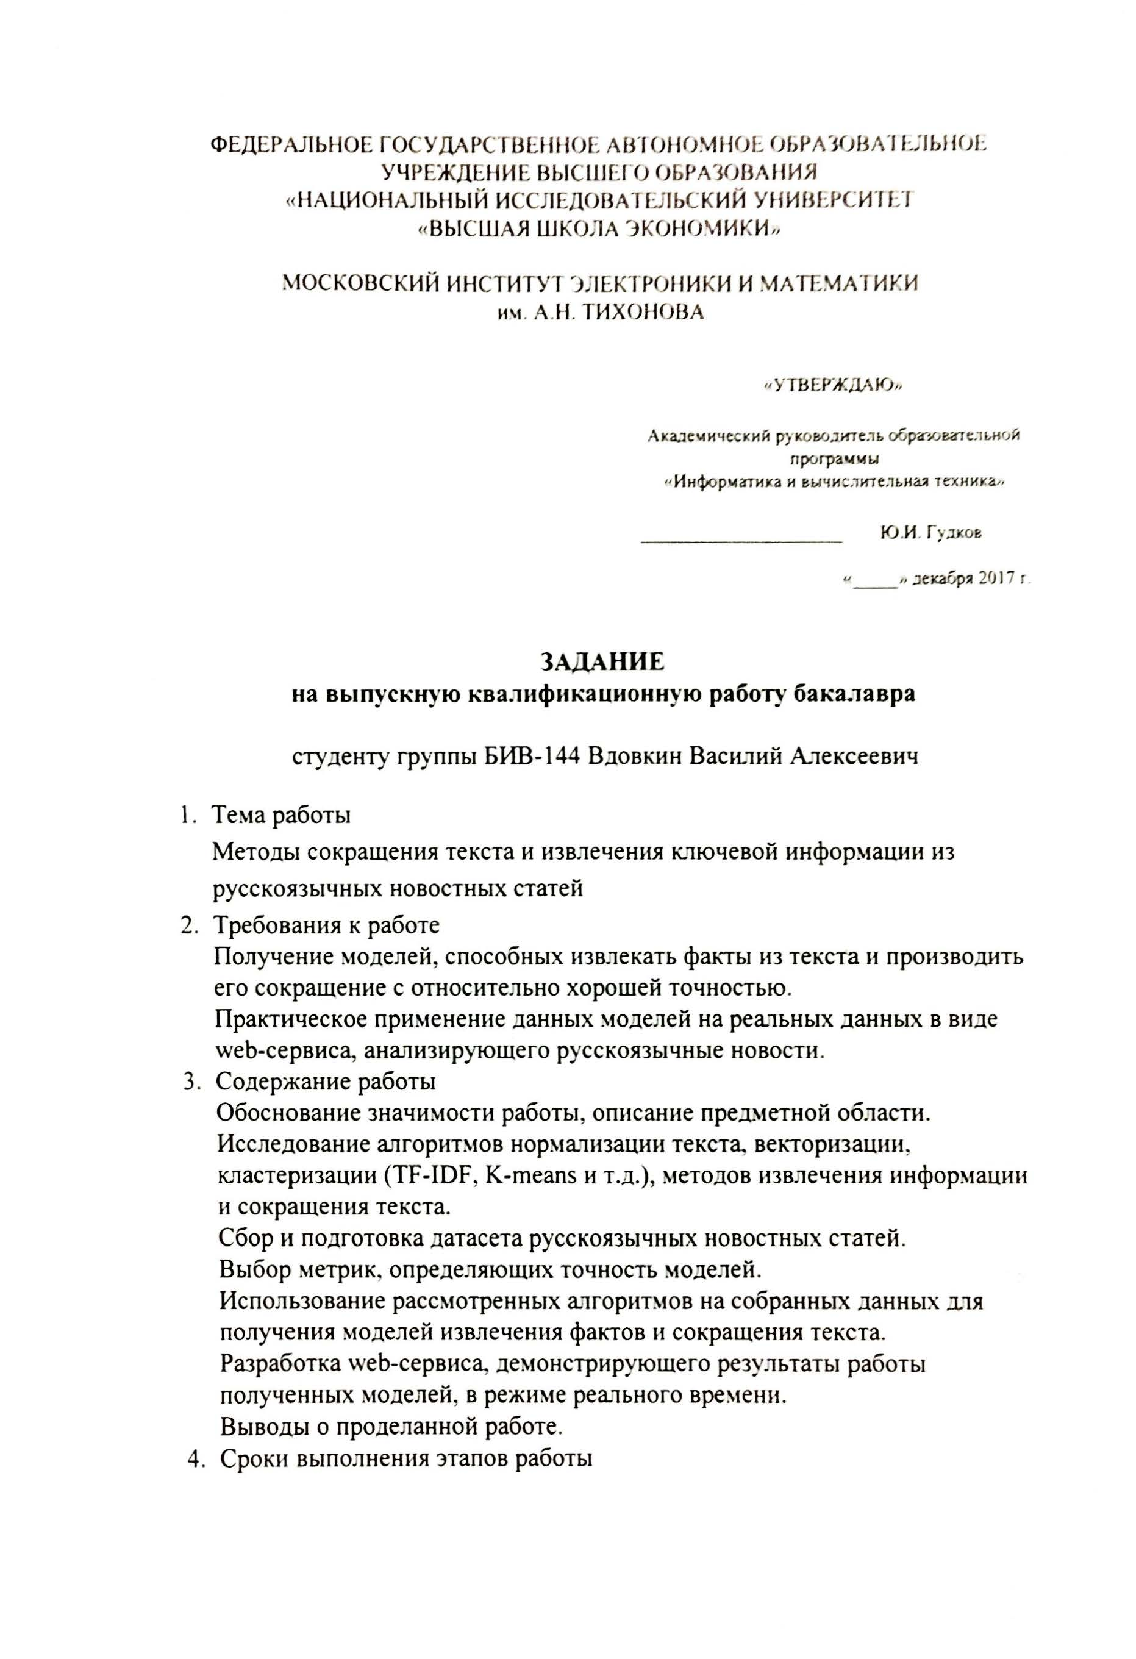
\includepdf[pages=-]{nott.pdf}

\begin{titlepage}
	\begin{center}
		ФЕДЕРАЛЬНОЕ ГОСУДАРСТВЕННОЕ АВТОНОМНОЕ
		
		ОБРАЗОВАТЕЛЬНОЕ УЧРЕЖДЕНИЕ ВЫСШЕГО ОБРАЗОВАНИЯ
		
		<<НАЦИОНАЛЬНЫЙ ИССЛЕДОВАТЕЛЬСКИЙ УНИВЕРСИТЕТ
		
		<<ВЫСШАЯ~ШКОЛА~ЭКОНОМИКИ>>
		\vspace{1cm}
		
		МОСКОВСКИЙ ИНСТИТУТ ЭЛЕКТРОНИКИ И МАТЕМАТИКИ\\  
		им. А.Н. ТИХОНОВА
		\vspace{1cm}
		
		Вдовкин Василий Алексеевич, группа БИВ-144
		
		\vspace{1cm}
		
		\MakeUppercase{\textbf{Методы сокращения текста и извлечения ключевой информации из русскоязычных новостных статей}}
		
		\vspace{1cm}
		
		Выпускная квалификационная работа 
		
		по направлению 09.03.01 Информатика и вычислительная техника 
		
		студентов образовательной программы бакалавриата
		
		<<Информатика и вычислительная техника>>
		
	\end{center}
  	\vspace{1cm}
  	\begin{flushright}
  		Студент~\rule{4cm}{.1pt}~В.А.\,Вдовкин
  	\end{flushright}
  	\vspace{1cm}
  	\begin{flushleft}
  		Рецензент \hfill  Руководитель
  		
  		к.т.н., доцент \hfill старший преподаватель
  		
  		?.?. ???? \hfill Ф.В.\,Волкова
  		
  		\rule{4cm}{.1pt} \hfill \rule{4cm}{.1pt}
  		
  	\end{flushleft}
  	\vfill\center{Москва 2018 г.}
\end{titlepage} % Титульник
\titleformat{\section}[block]
{\centering\fontsize{16pt}{18pt}\selectfont\bfseries}{\thesection\cftsecaftersnum}{0.5em}{} % по центру

\section*{Аннотация}
Данная работа описывает процесс реализации сервиса, способного значительно улучшить
и упростить пользовательское взаимодействие с новостным контентом, используя обработку
естественного языка (Natural Language Processing, NLP). Сервис анализирует поток русскоязычных новостных статей в реальном времени, группирует их по конкретным событиям и выделяет ключевую информацию о событии.
Для построения такого сервиса мы изучаем и используем различные методы и модели, распространенные в NLP для решения следующих задач:
нормализация, векторизация, кластеризация и суммаризация текста.
Кластеризация используется для выделения из потока данных множества статей, относящемся к одному событию.
Мы собираем и обрабатываем большое количество данных с web-сайтов медиа и обучаем векторизатор TF-IDF, позволяющий использовать K-means для кластеризации.
Суммаризация извлекает самые информативные предложения из кластера-события и формирует параграф из 5 следующих по смыслу предложений. Для суммаризации используются две модели: SimBasic и DivRank. Выбранные решения сравниваются и оцениваются.


\section*{Abstract}
This work describes implementation of the service that can significantly improve user experience in news content consumption by using Natural Language Processing (NLP for short). This service analyses stream of news articles from russian media web-sites in real-time, groups news by events and extracts the most valuable information about the events.
To implement this service we first research and then use models and methods from NLP to find suitable solution for the following problems: normalization, vectorization, clusterization and summarization of text.
Clusterization allows us to automatically group news by events. In order for this to work, we collect the data from web-sites of media and train TF-IDF model allows to use K-means algorithm for news clusterization. Summarization depends on SimBasic and DivRank models and extracts the most informative sentences from the event-cluster. We compare and evaluate the proposed solutions.

\titleformat{\section}[block]
{\raggedright\fontsize{16pt}{18pt}\selectfont\bfseries}{\thesection\cftsecaftersnum}{0.5em}{} % справа % Аннотация
\tableofcontents % Оглавление 
\clearpage

\section{Введение}


Когда в мире происходит какое-либо событие, различные средства массовой информации
пишут статьи с информацией о нём в виде новостей. Пользователю часто бывает сложно ориентироваться в большом потоке данных от разных источников. Автоматическая систематизация и обработка таких данных с целью предоставить наиболее полную и информативную картину может сэкономить человеку много времени. 

Человек очень просто понимает информацию, содержащуюся в тексте на естественном языке, потому что он учится этому с рождения, не заметно для себя, выучивая связи между устройством языка и информацией, которую с помощью него передают. С другой стороны, формализация этих правил очень сложна для людей, поэтому на ней сосредоточено множество разделов лингвистики. Сейчас редакторы новостных медиа почти полностью вручную выполняют все задачи, связанные с текстом: размечают теги, собирают подборки и, чаще всего, <<генерируют>> новости полностью опираясь статьи-источники.

С помощью математических моделей, описывающих связи между информацией и естественным языком, можно автоматизировать эти процессы. В последнее десятилетие быстрыми темпами развивается обработка естественного языка (Natural Language Processing, NLP), которая с помощью моделей и алгоритмов решает задачи автоматического анализа текста, в частности, объединение новостных статей в группы (кластеры) по релевантности к конкретному событию (кластеризация), извлечение из кластера наиболее информативных данных о событии, например, в виде нескольких предложений. Самые базовые и повседневные интернет-сервисы построены с использованием NLP: поиск, таргетинговая реклама, рекомендательные сервисы и т.п.

{\bf Целью выпускного проекта} является разработка веб-сервиса, который автоматически
группирует русскоязычные новостные статьи по событиям и извлекает из них ключевую информацию в режиме реального времени. 

Для достижения данной цели необходимо решить {\bf следующие задачи}:
\begin{enumerate}
	\item Реализация системы сбора данных: сбор статей (парсинг) с web-сайтов СМИ для получения новостей вместе с их метаданными.
	\item Изучение алгоритмов и моделей анализа текста: нормализация, векторизация, кластеризация и суммаризация.
	\item Изучение технической реализации модуля анализа текста.
	\item Проектирование и разработка инфраструктуры сервиса, интеграция с ранее реализованными модулями сбора и анализа данных.
	\item Оценка качества сервиса, анализ предложенных решений и выводы.
\end{enumerate}


\section{Данные}
Многие NLP модели требуют большого количества предварительно обработанных данных для обучения, в частности TF-IDF векторизатор. В данном случае такими данными является корпус русскоязычных новостей. В исследовательских работах авторы часто используют готовые данные, например, общедоступные размеченные датасеты, но если учитывать цель проекта, то без реализации своей системы, позволяющей получать новости с нескольких источников за определённый период времени, не обойтись.

С помощью собственной системы парсинга собран датасет, состоящий из нескольких сотен тысяч новостных статей с сайтов следующих СМИ: <<Новая газета>>, <<Газета.Ru>>, <<Lenta.ru>>, <<ТАСС>>, <<ВЕДОМОСТИ>>, <<Медуза>>, <<РИА Новости>> с метаданными (заголовок, текст, дата, тема). При обработке выяснилось, что у многих статей темы указаны некорректно (например, у <<РИА Новостей>> большая половина контента помечена тегом <<проишествие>>, у <<Новой газеты>> все новости старее 2014 года~--- тегом <<политика>>). После чистки данных в датасете осталось 130 тыс. документов, имеющих 32 различных тега. Распределение тегов и источников показано на рис. \ref{datadistr}.

\begin{figure}[h!]
	\centering
	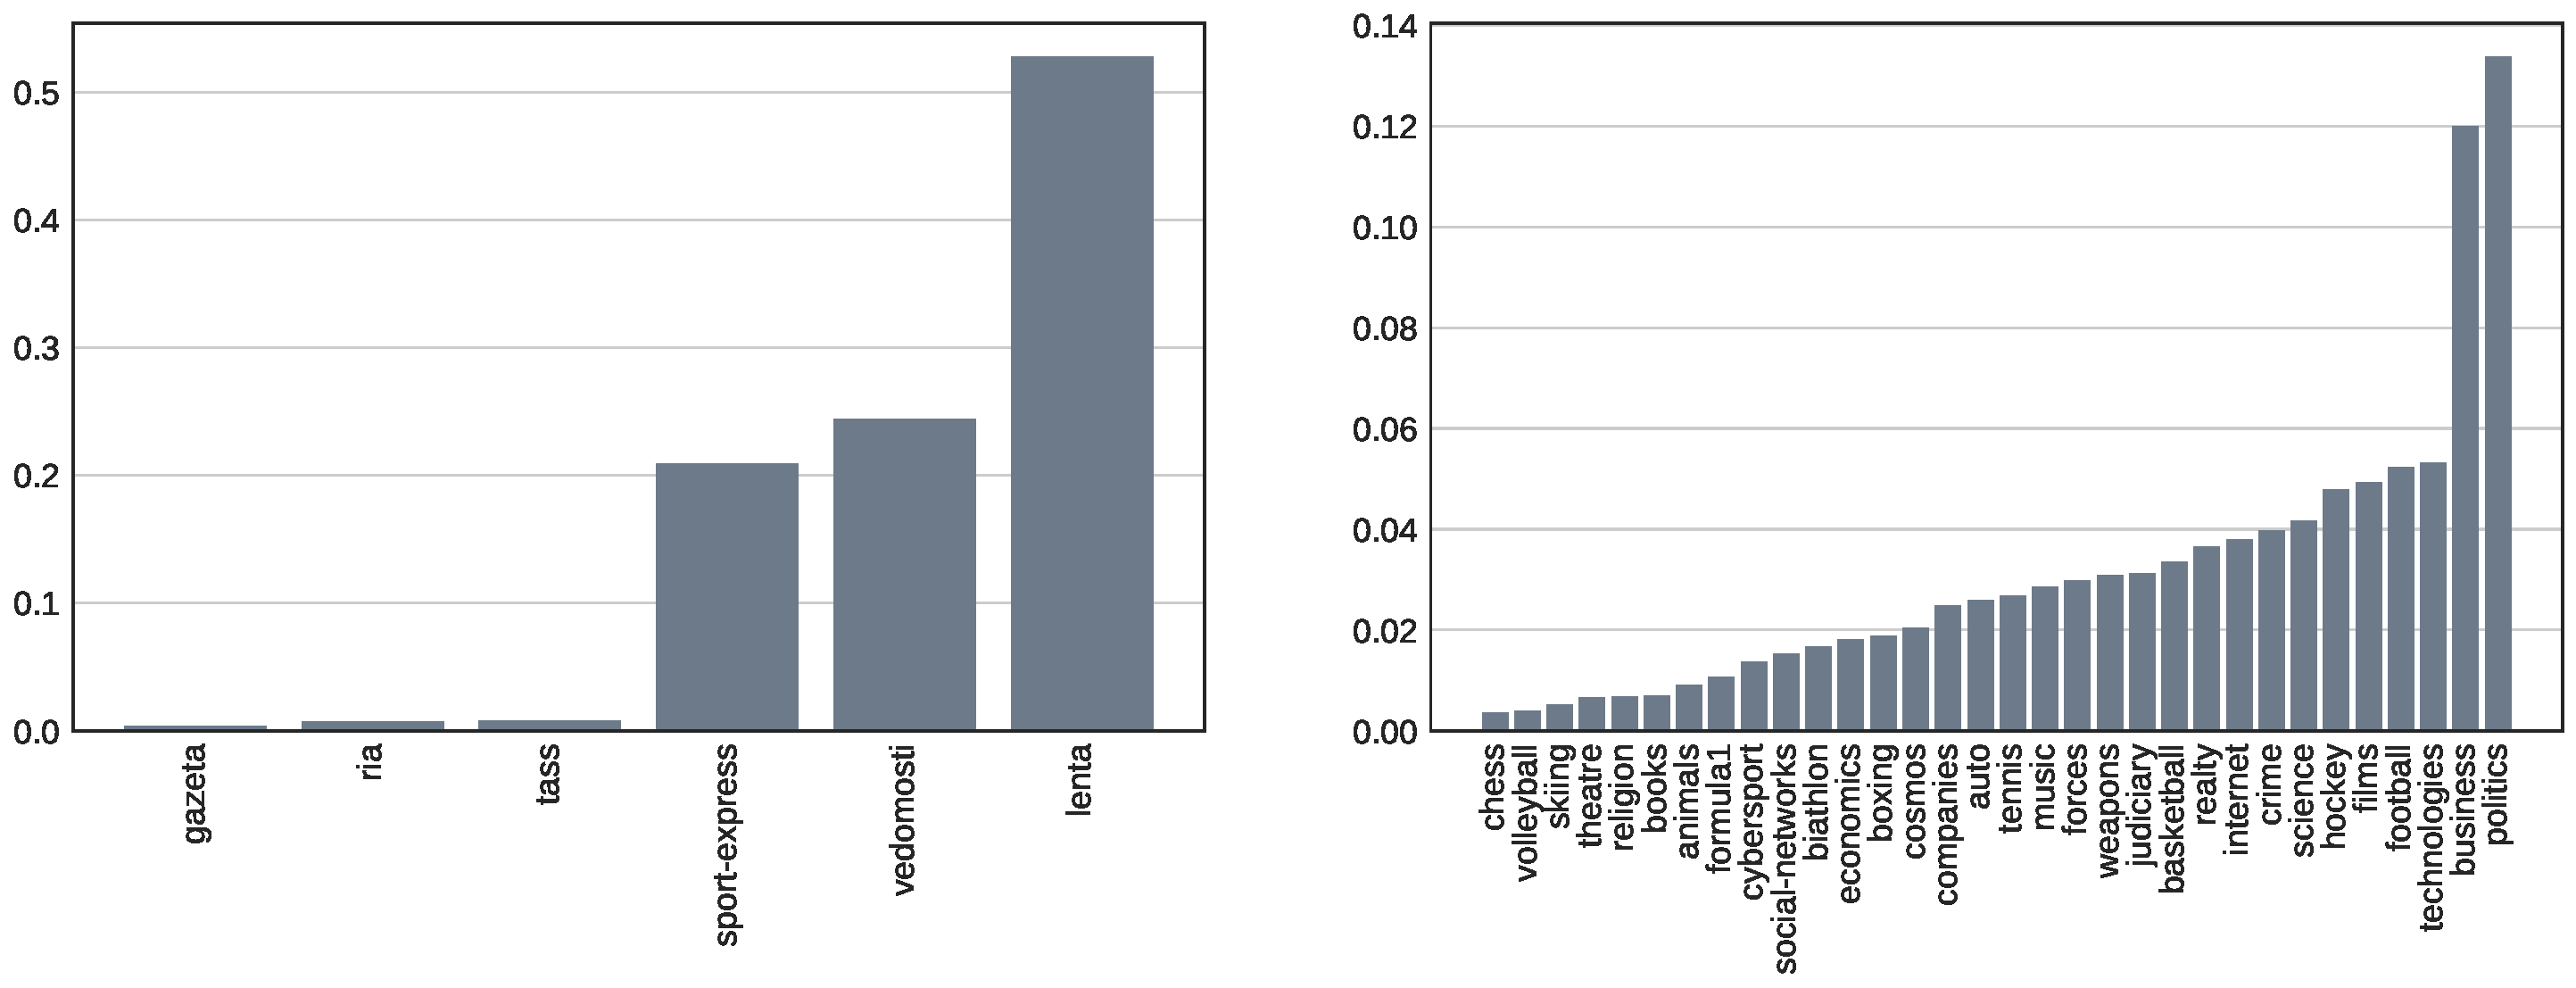
\includegraphics[scale=0.35]{datadistr}
	\caption{Распределение тегов и источников в датасете статей для обучения TF-IDF векторизатора.}
	\label{datadistr}
\end{figure}

От объективности данного датасета зависит качество всего сервиса, так как на нём обучается векторизатор TF-IDF, на котором основан алгоритм кластеризации, а от него, в свою очередь, зависит суммаризация события. Для проверки валидности данных и обученного векторизатора реализован классификатор SVM (support vector machine).

SVM методы классификации используют операции линейной алгебры при работе с векторизованым текстом, при обучении <<пытаясь>> разделить многомерное пространство так, чтобы максимальное количество точек  (векторов) одного и того же класса находилось в одной части пространства. Это можно достичь с помощью перехода к $n+1$-мерному пространству, как условно показано на рис. \ref{svm_cond}.

\begin{figure}
	\centering
	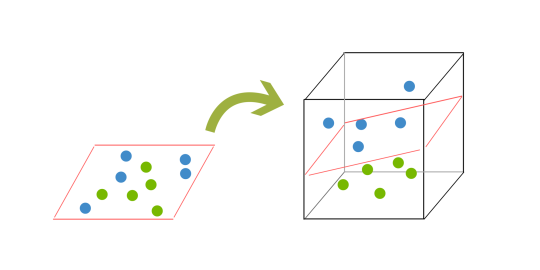
\includegraphics[scale=0.6]{svm_cond}
	\caption{Явное разделение данных на два класса при переходе в пространство более высокой размерности.}
	\label{svm_cond}
\end{figure}

SVM классификаторы очень популярный инструмент в NLP задачах, поэтому существует множество реализаций с полезными функциями. Мы использовали его модификацию \verb+SGDClassifier+, которая оптимизирует параметры с помощью градиентного спуска.

Проверка валидности состоит в эмпирической оценке признаков классов~--- это самые <<весомые>> слова, больше всего влияющие на принадлежность к конкретному классу. При изучении слов-признаков из таблицы \ref{word_feachers} видно: слова-признаки и слова-классы связаны по смыслу и, в некоторых случаях, являются синонимами, что свидетельствует о корректности данных и векторизатора. Метрики качества классификаторы тоже поддтверждают правильность датасета: $\text{Accuracy} = 0,8687$, $\text{F1 score} = 0,8711$, матрица ошибок представлена в приложении на рис. \ref{svm_matrix}.

\begin{table}
	\caption{Слова-признаки для собранного датасета.}
	\resizebox{\textwidth}{!}{%
		\begin{tabular}{r|cccccccc}
			\textbf{animals}         &               жить &          вольер &             хозяин &              животный &               зоопарк &        питомец &           кличка &        животное \\
			\textbf{auto}            &          авторынок &           осаго &      автомобильный &     автопроизводитель &              автопром &          камаз &          автоваз &      автомобиль \\
			\textbf{basketball}      &                рфб &      евробаскет &          центровой &          кубок европа &             баскетбол &   баскетболист &         евролига &             нба \\
			\textbf{biathlon}        &           эстафета &    биатлонистка &            шипулин &                   сбр &            хохфильцен &        биатлон &              ibu &      биатлонист \\
			\textbf{books}           &         библиотека &    произведение &       писательница &                 роман &                 книга &   литературный &             поэт &        писатель \\
			\textbf{boxing}          &              алоян &          лебзяк &                мма &              поединок &              поветкин &            бой &             бокс &          боксер \\
			\textbf{business}        &   россельхознадзор &            fifa &                ржд &               газпром &           туроператор &        formula &         ритейлер &             оао \\
			\textbf{chess}           &            карякин &       шахматист &           карякина &                магнус &               шахматы &        карлсен &              фид &       шахматный \\
			\textbf{companies}       &  тысяча автомобиль &        компания &  миллиард кубометр &              миллиард &                тысяча &  процент акция &         ретейлер &         процент \\
			\textbf{cosmos}          &          космонавт &         светить &           прогресс &             вселенная &                космос &     астрофизик &             марс &       астронавт \\
			\textbf{crime}           &          грабитель &         изымать &        группировка &               полиция &               убивать &         летний &       преступник &          тюрьма \\
			\textbf{cybersport}      &             gaming &            team &              valve &           киберфутбол &                  dota &     киберспорт &  киберспортивный &  киберспортсмен \\
			\textbf{economics}       &               мрот &          греция &             бюджет &                пенсия &                   ввп &         минфин &        экономика &        инфляция \\
			\textbf{films}           &         мультфильм &          сериал &            актриса &                  кино &               картина &       режиссер &            актер &           фильм \\
			\textbf{football}        &               поле &         стадион &         нападающий &              матч тур &                  фифа &           уефа &        футболист &    полузащитник \\
			\textbf{forces}          &       развертывать &      выполнение &     военнослужащий &               военный &                 шойгу &        генштаб &       конашенков &      минобороны \\
			\textbf{formula1}        &              манор &      цитировать &               рено &               феррари &              макларен &          пилот &         мерседес &         формула \\
			\textbf{hockey}          &           авангард &             ска &              шайба &            нападающий &                хоккей &       хоккеист &              нхл &             кхл \\
			\textbf{internet}        &          википедия &          сервис &             ресурс &               youtube &                  сайт &          хакер &           блогер &        интернет \\
			\textbf{judiciary}       &             стража &          статья &       арестовывать &               колония &  следственный комитет &      следствие &              скр &  комитет россия \\
			\textbf{music}           &         композитор &     евровидение &              песня &                 певец &               концерт &         альбом &           певица &        музыкант \\
			\textbf{politics}        &              лидер &          кремль &      парламентарий &                партия &               депутат &        госдума &            глава &             мид \\
			\textbf{realty}          &             объект &    строительный &           жилищный &         строительство &                   жкх &        ипотека &            жилье &    недвижимость \\
			\textbf{religion}        &          монастырь &           собор &          церковный &                муфтий &                святой &       христиан &       митрополит &        патриарх \\
			\textbf{science}         &        университет &          журнал &          математик &                 физик &               научный &       археолог &    исследователь &          ученый \\
			\textbf{skiing}          &             вяльбе &          нортуг &             лыжник &                   fis &                легков &         йохауг &            лахти &         устюгов \\
			\textbf{social-networks} &          некоторые &            юзер &           facebook &               twitter &     пользователь сеть &   пользователь &        вконтакте &         соцсеть \\
			\textbf{technologies}    &          vimpelcom &           apple &           оператор &                  wifi &              говорить &            мтс &            робот &         контакт \\
			\textbf{tennis}          &    кубок федерация &            open &            шарапов &                теннис &                  корт &      теннисист &      теннисистка &     кубок дэвис \\
			\textbf{theatre}         &         росгосцирк &        цирковой &              балет &            постановка &           театральный &         мюзикл &            театр &       спектакль \\
			\textbf{volleyball}      &              факел &         маричев &             алекно &             суперлига &             казанский &      белогорье &      волейболист &        волейбол \\
			\textbf{weapons}         &               jane &  использоваться &       defense news &  министерство оборона &             миллиметр &  миллиметровый &          defense &             тип \\
		\end{tabular}
		}
	\label{word_feachers}
\end{table}


\section{Анализ текста}
\subsection{Нормализация}

Текст на естественном языке содержит много избыточных элементов, без которых его смысл не изменится. Чаще всего они действуют как <<шум>>, так как встречаются равномерно по всему корпусу языка. Подобными элементами почти всегда выступают союзы, предлоги, части слов, отвечающие за форму. Кроме того, существуют разные способы написания одних и тех же объектов, например, числительные можно написать цифрами. При решении любой задачи в NLP текст нормализуют, то есть приводят в общую, более информативную форму, без <<шума>>. Нормализация включает в себя несколько шагов.

При работе с естественной информацией её дискретизуют. Похожий процесс в NLP называется токенизация, он заключается в делении текста на части~--- токены, обычно токен является одним словом. К сожалению, просто делить текст по пробелам не совсем корректно, так как существует множество исключений, например, Великие Луки~--- это один токен, хотя и состоит из двух слов. Если рассматривать это как два токена, то смысл текста будет искажён, что может сказаться на результате и на качестве решения задачи. Для токенизации удобно использовать регулярные выражения.

В данном проекте используется два токенизатора: простое деление на слова при обработке текста для TF-IDF и Punkt токенизатор для деления статей на предложения при суммаризации. Последний использует корпус для обучения без учителя, <<выучивая>> последовательности, с которых начинаются предложения, что помогает работать с нелитературными данными, например, сообщениями в соц. сетях, где предложения часто начинаются с маленькой буквы.

Следующий шаг нормализации~--- удаление стоп-слов. Стоп-слова примерно одинаково распределены по всему корпусу языка. В русском языке ими являются многие служебные части (союзы, междометия, предлоги).

Для однозначной идентификации слова его приводят к начальной форме. Данный процесс называется лемматизация, а начальная форма~--- лемма. Для лемматизации недостаточно использовать только словарь, потому что существует огромное количество неологизмов, подчиняющимся тем же морфологическим правилам при образовании форм. Хорошие лемматайзеры проводят полный морфологический парсинг, при котором слова делятся на морфемы: стемы (самые осмысленные части) и афиксы (придают дополнительное значение слову). Более простая версия морфологического анализа~--- стемминг, использующий определённые правила для извлечения основы слова.

Мы используем лемматизатор MyStem, предоставляющий универсальный для многих языков алгоритм морфологического разбора, использующийся в популярном поисковом движке \cite{pystem}.
%https://cache-mskm910.cdn.yandex.net/download.yandex.ru/company/iseg-las-vegas.pdf

При обработке данных перед векторизаций последовательно выполняются следующие операции:
\begin{enumerate}
	\item приведение текста в нижний регистр;
	\item удаление символов пунктуации;
	\item удаление стоп-слов.
	\item лемматизация каждого слова с помощью Python библиотеки MyStem.
\end{enumerate}
 Примеры предложений после перечисленных действий представлены в таблице \ref{exa}.


\begin{table}
	\centering
	\caption{Примеры нормализации текста}
	\resizebox{\textwidth}{!}{%
		\begin{tabular}{|l|l|}
			\hline
			Оригинал  & Нормализация \\ \hline\hline
			\makecell[l]{Однако когда их проверили на восприятие\\ концепций и идей, оказалось, что те, \\кто писал от руки, понимают пройденный \\материал лучше однокашников.} & \makecell[l]{однако когда они проверять на восприятие \\концепция идея оказываться что тот \\кто писать от рука понимать проходить\\ материал хорошо однокашник}
			\\ \hline
			\makecell[l]{Лингвистическую относительность упоминали\\ в своих сочинениях немецкие философы\\ еще в конце XVIII – начале XIX века, \\но известность гипотеза получила\\ именно благодаря Уорфу.} & \makecell[l]{лингвистический относительность упоминать \\свой сочинение немецкий философ \\еще конец xviii – начало xix век \\но известность гипотеза получать\\ именно благодаря уорфу} \\ \hline
		\end{tabular}
	}
	\label{exa}
\end{table}


\subsection{Векторизация}

TF-IDF --- статистическая мера, используемая для оценки важности слова в любом контексте, основанная на его встречаемости в документе. Чем реже слово появляется в документе, тем выше его TF-IDF вес \cite{doi:10.1108/eb026526}.

TF-IDF --- это произведение двух статистик: TF (term frequency) и IDF (inverse 
document frequency). 

Существует несколько способов подсчёта TF-IDF, в данной работе использовался следующий:
$$
\text{tf}(t, d) = \cfrac{n_t}{\sum_{k} n_k},
$$
где $n_{t}$ есть число вхождений слова $t$ в документ, а $\sum_{k} n_k$ --- общее число слов в данном документе.

$$
\text{idf}(t, D) = \log{ \cfrac{|D|}{|\{ d_i \in D \mid t \in d_i \}|}},
$$
где $|D|$ --- число документов в корпусе, $|\{ d_i \in D \mid t \in d_i \}|$ — число документов из корпуса $D$, в которых встречается 
$t$ (когда $n_{t} \neq 0$).

Таким образом, мера TF-IDF является произведением двух сомножителей:
$$
\text{TF-IDF}(t, d, D) = \text{tf}(t, d) \cdot \text{idf}(t, D).
$$

Признаковым описанием одного объекта $d \in D$ будет вектор
$$
\big(\text{TF-IDF}(t,d,D)\big)_{t\in V},
$$
где $V$ --- словарь всех слов, встречающихся в корпусе $D$.

Обучение модели заключается в подсчёте веса каждого уникального слова в каждом документе.

Одно из полезных свойств векторов TF-IDF: косинусное расстояние между векторами характеризует <<похожесть>> статьей, что можно использовать для кластеризации.

\subsection{Кластеризация}
Самый базовый алгоритм кластеризации, который в данном случае применим~--- алгоритм поиска связных компонентов в графе. Его псевдокод показан на рис. \ref{pseudo}, где $V, E$~--- множество вершин и рёбер графа, $(u,v),(u,n)$~--- рёбра, $v,u,n$~---вершины, 
$w(u,v)$~--- вес ребра $(u,v)$, $c[v]$~--- номер компоненты (кластера) вершины $v$, $Q$~--- очереди вершин для посещения, $S$ множество посещённых вершин, $compNum$~--- номер текущей компоненты.

\begin{figure}
	\begin{algorithm}[H]
		\DontPrintSemicolon
		$ compNum \gets 0 $\;
		\For{$(u,v) \in E$}{
			$w(u,v) \gets \cos{(u,v)}$\;
		}
		\For{$v \in V$}{
			$c[v] \gets  nil $\;
		}
		\For{$v \in V$}{
			\If{$ c[v] = nil $} {
				$ c[v] \gets compNum $\;
				$Q \gets \{v\}$\;
				$S \gets \emptyset$\;
				\While{ $ Q \ne \emptyset$}{
					$u \gets pop(Q)$\;
					$c[u] \gets compNum$\;
					$S \gets S \cup \{v\}$\;
					\For{$n \notin S, (u,n) \in E$}{
						\If{$w(u, n) \geqslant \text{threshold}$ {\bf and} $c[n] = nil $} {
							$Q \gets Q \cup \{n\}$\;
						}
					}
				}
				$ compNum \gets compNum + 1 $
			}
		}
	\end{algorithm}
	\caption{Псевдокод графовой кластеризации.}
	\label{pseudo}
\end{figure}

Алгоритм работает следующим образом: строится полный граф, значения ребёр выставляется как косинусное расстояние между векторами-вершинами. Далее, от каждой не помеченной номером кластера вершины запускается BFS алгоритм (breadth-first search, поиск в ширину), игнорирующий рёбра меньше определённого значения, и устанавливающий номер своего кластера любой вершине, которой удалось достичь. Этот процесс повторяется до тех пор, пока всем вершинам не назначен номер кластера.

Данный алгоритм очень прост в реализации и показывает хорошие результаты, кроме того, ему не нужно чзаранее знать количество кластеров, единственный параметр threshold~--- порог, ниже которого рёбра игнорируются.


Другой, более популярный, но не менее простой алгоритм кластеризации K-means рассматривает векторы, как точки в пространстве, выбирает $k$ случайных точек-центроидов и все ближайшие к ним точки-вектора статей, формируя $k$ случайных групп  (рис. \ref{km}, б). Далее у каждой группы определяется средняя точка, которая становится новым центроидом (рис. \ref{km}, в). Процесс повторяется до тех пор, пока точки не перестанут сдвигаться (рис. \ref{km}, г--e).

\begin{figure}
	\centering
	\begin{subfigure}[b]{0.3\textwidth}
		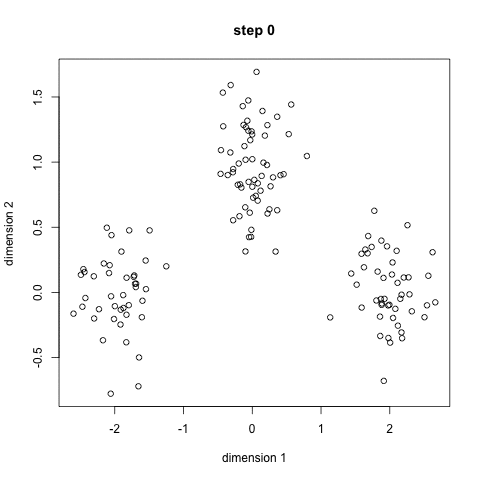
\includegraphics[width=\textwidth]{k_0}
		\caption{}
	\end{subfigure}
	~
	\begin{subfigure}[b]{0.3\textwidth}
		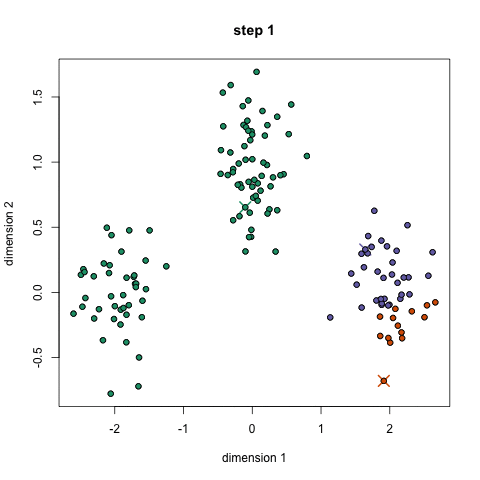
\includegraphics[width=\textwidth]{k_1}
		\caption{}
	\end{subfigure}
	~ 
	\begin{subfigure}[b]{0.3\textwidth}
		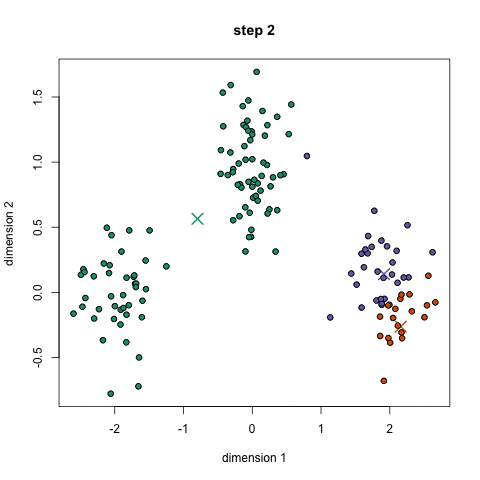
\includegraphics[width=\textwidth]{k_2}
		\caption{}
	\end{subfigure}
	~ 
	
	\begin{subfigure}[b]{0.3\textwidth}
		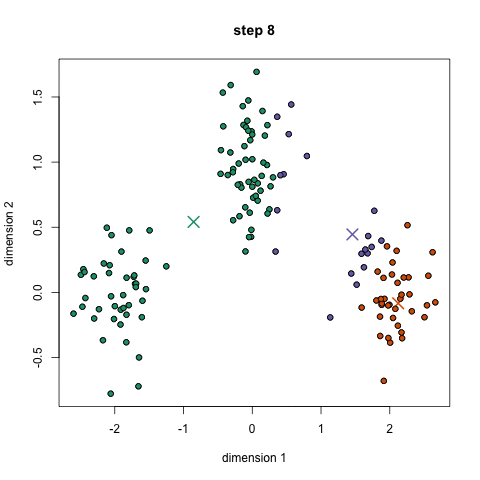
\includegraphics[width=\textwidth]{k_3}
		\caption{}
	\end{subfigure}
	~
	\begin{subfigure}[b]{0.3\textwidth}
		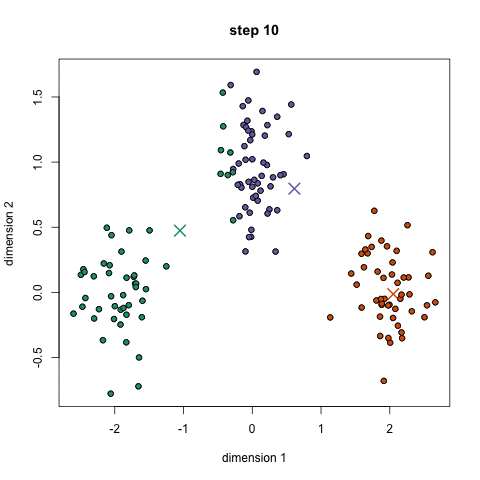
\includegraphics[width=\textwidth]{k_4}
		\caption{}
	\end{subfigure}
	~ 
	\begin{subfigure}[b]{0.3\textwidth}
		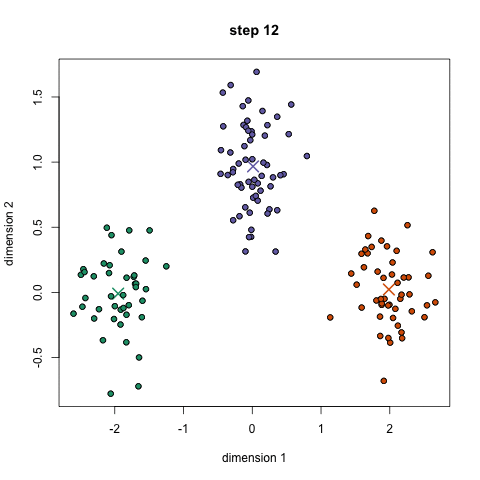
\includegraphics[width=\textwidth]{k_5}
		\caption{}
	\end{subfigure}
	\caption{Визуализация кластеризации K-means.}
	\label{km}
\end{figure}

В проекте используется алгоритм K-means, так как при эмпирическом сравнении он показывает результаты чуть лучшие графового подхода и имеет больше параметров, что позволяет его тонко настроить в зависимости от размера данных. Если данных для кластеризации очень много, как это часто бывает, то алгоритму может не хватить оперативной памяти. Для решения этой проблемы существует вариант K-means, принимающий данные по частям (batches), к сожалению, время работы алгоритма при этом увеличивается в зависимости от размера частей.



\subsection{Суммаризация}
Алгоритмы суммаризации можно условно поделить на две группы: абстрактная (abstractive) и извлекающая (extractive). Первая генерирует текст по смыслу, вторая выбирает самые информативные предложения из исходного текста и склеивает их. Модели абстрактной суммаризации требуют больших вычислительных мощностей и сложны в реализации, так как основаны на нейронных сетях, при их использовании стоит учитывать особенности языка и использовать эвристики для генерации корректных форм слов или словосочетаний. Извлекающая суммаризация легче в реализации и выглядит правдоподобно, так как состоит из написанных человеком предложений.

В сервисе используются два алгоритма MDS (multi-document summarization): SumBasic и DivRank, подразумевающие суммаризацию сразу нескольких документов на одну тему, что хорошо подходит для кластеров-событий.
  
\subsubsection{SumBasic}
SumBasic основан на простом наблюдении: слова, появляющиеся часто в кластере документов, с большей вероятностью окажутся в сокращённых текстах, написанных человеком, чем остальные.

Алгоритм SumBasic состоит из следующих шагов:
\begin{enumerate}
	\item Для каждого уникального слова $w_i$ посчитать вероятность его присутствия во входных данных $p(w_i)=\frac{n}{N}$, где $n$~--- количество вхождений слова $w_i$ в данных, а $N$~--- общее количество слов.
	\item Взвесить каждое предложение $S_j$, посчитав среднюю вероятность $p(w_i)$:
	$$ weight(S_j) = \sum_{w_i\in S_j} \frac{p(w_i)}{|\{w_i|w_i\in S_j\}|}$$
	\item Выбрать предложение с лучшим весом, содержащие слово с максимальной вероятностью.
	\item Для каждого слова $w_i$ в выбранном предложении обновить их вероятность:
	$$p_{new}(w_i) = p_{old}(w_i)^2$$
	\item Если уже выбранных предложений недостаточно перейти на шаг 2. 
\end{enumerate} 

Шаг 3 гарантирует, что предложение с самым вероятным словом будет выбрано. Шаг 4 добавляет алгоритму <<чувствительность>> к контексту сокращения: обновляя вероятности таким образом мы позволяем изначально невероятным словам оказывать большее влияние на выбор предложений, и, самое главное, этот шаг позволяет эффективно применять алгоритм для нескольких документов, позволяя игнорировать уже сокращённую информацию, реализуя <<затухание>> вероятности слов \cite{Nenkova05theimpact, Vanderwende07beyondsumbasic}.

SumBasic выбран из-за его простоты и элегантности для сравнения с более сложным алгоритмом DivRank.
\subsubsection{DivRank}

DivRank (Diverse Rank)~--- алгоритм для взвешивания графов, подобный популярному PageRank, но применяющийся для MDS суммаризации. Для его использования необходимо построить граф, схожий с тем, что описан в графовом методе кластеризации в п.3.3. Различия в том, что здесь вершины~--- это TF-IDF вектора предложений, а не статей. Рёбра удаляются, если косинусное расстояние меньше 0.1. После взвешивания этого графа DivRank'ком выбираются $k$ первых самых весомых предложений.

На рис. \ref{div}, в показан <<разнообразно>> взвешенный граф с помощью DivRank в сравнении с графом, взвешенный используя PageRank (рис. \ref{div}, б). Если необходимо выбрать 3 вершины, максимально и ёмко передающие информацию о графе, то алгоритм DivRank выдаст вершины 1,4,5, что даже визуально лучше, чем ответ алгоритма 1,2,3 PageRank \cite{Mei10divrank:the}. 
\begin{figure}[h]
	\centering
	\begin{subfigure}[b]{0.3\textwidth}
		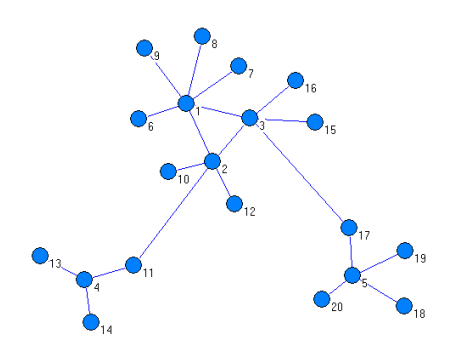
\includegraphics[width=\textwidth]{NoR}
		\caption{Исходный граф}
	\end{subfigure}
	~
	\begin{subfigure}[b]{0.3\textwidth}
		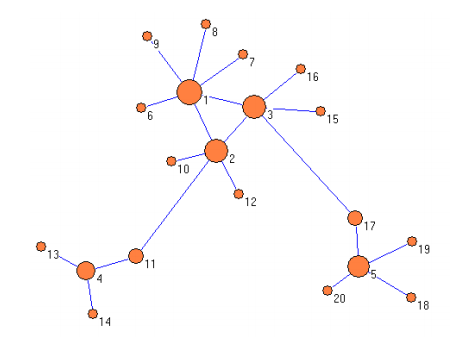
\includegraphics[width=\textwidth]{PageR}
		\caption{PageRank}
	\end{subfigure}
	~ 
	\begin{subfigure}[b]{0.3\textwidth}
		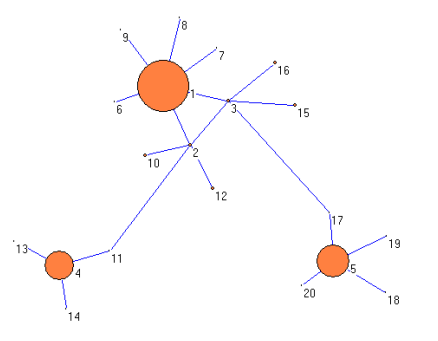
\includegraphics[width=\textwidth]{DivR}
		\caption{DivRank}
	\end{subfigure}
	\caption{Взвешивание графа}
	\label{div}
\end{figure}


\section{Реализация сервиса}
\subsection{Архитектура и транспорт данных}
Сервис представляет из себя 4 обособленных docker-контейнера взаимодействующие между собой путём обмена json-объектами с помощью базы данных Mongodb.

Контейнеры по порядку развертывания сервиса:
\begin{enumerate}
	\item {\it mongo}~--- база данных. Запускается мнгновенно.
	\item {\it getter}~--- сервис парсинга. Запускается мнгновенно, пишет в коллекцию \texttt{raw\_news} базу данных новости за последние несколько часов при инициализации. Если при запуске в коллекции остались старые необработанные новости, они удаляются.
	\item {\it analyser}~--- сервис анализа текста. Запускается через несколько десятков секунд после деплоя, ожидая данные от {\it getter}. Читает из коллекции \texttt{raw\_news}, удаляя из неё каждую обработанную новость. Пишет в коллекцию \texttt{events}. Если при запуске в коллекции находятся старые данные, они не удаляются, чтобы сервер отдавал их, а не пустоту по время развёртывания.
	\item {\it server}~--- выступает в роли интерфейса, отдаёт пользователю обработанные данные сервиса.
\end{enumerate}

Деплой происходит с помощью docker-compose. Для быстрой установки и развёртывания написан скрипт (рис. \ref{bash}).

Все контейнеры, кроме базы данных, могут функционировать независимо друг от друга, что очень полезно при разработке. Все приложения внутри реализованы на Python 3.

\begin{figure}
	\centering
\begin{minted}[fontsize=\small]{python}
sudo apt install docker.io
sudo docker login -u ... -p ...
sudo pip install docker-compose
cd app/analyzer/nlp/models
wget "https://www.dropbox.com/sh/8s9qfy5rf1o5bbd/AAAVSVQZorVr6JH8LPJQX9tva?dl=1" \
-O models.zip && unzip models.zip -x /
cd app
sudo docker-compose build
sudo docker-compose up -d
sudo docker-compose logs -f
\end{minted}
	\caption{Скрипт для запуска сервиса с установкой необходимых компонентов.}
	\label{bash}
\end{figure}


\subsection{Особенности реализации компонентов анализа}
\subsubsection{Система сбора данных}

Система сбора данных представляет собой коллекцию парсеров сайтов российских СМИ, основанные на одном подходе и имеющие одинаковый интерфейс.

Чтобы понять, как реализовать универсальную систему, с возможностью быстрого добавления поддержки нового ресурса, достаточно взглянуть на сайты русскоязычных медиа-ресурсов. Многие сильно отличаются друг от друга внешне, но у всех присутствует следующая логика: существуют страницы со списком новостей в хронологическом порядке, которые либо агрегированы по дням (Lenta.ru, Gazeta.ru, vedomosti.ru), либо используют параметр offset, указывающий с какой статьи начинать страницу (novayagazeta.ru, tass.ru, meduza.io). Первый вариант пагинации удобнее, потому что позволяет просто получить новости за любой заданный интервал времени. Во втором случае можно использовать бинарный поиск по страницам, но это не реализовано, так как новости всегда нужны с текущего момента.
Большинство СМИ отдают данные в HTML формате и только лишь малая часть использует API в JSON формате.

При инициализации сервиса необходимо получить новости за последние несколько часов, чтобы сформировать актуальные кластера, что занимает долгое время. Парсинг множества статей можно ускорить в несколько раз, обрабатывая их параллельно.

Так как система обособлена, то реализовывать её можно на любом языке, а взаимодействовать с сервисом через внешнее хранилище, но для удобства разработки выбран \texttt{Python 3}, с использованием дополнительных библиотек: 
\begin{itemize}
	\item \texttt{BeautifulSoup}~--- парсинг HTML.
	\item \texttt{multiprocessing}~--- распараллеливание задач.
	\item \texttt{pymongo}~--- интерфейс над внешним хранилищем Mongodb.
\end{itemize}

Так как Питон имеет ограничение на потоки из-за GIL, то чтобы обеспечить параллелизм, позволяющий с увеличением количества процессорных ядер ускорять обработку множества статей, используется модуль \texttt{multiprocessing}, что значительно усложняет задачу. Использование процессов вместо корутин и асинхронных задач в данном случае не даст большой прирост производительности, так как большинство процессорного времени тратиться не на чтение сокетов, а на парсинг HTML. 

Пример использования представлен на рис. \ref{example}. 

\begin{figure}
	\centering
	\begin{minted}[fontsize=\small]{python}
	from parsers import Gazeta, Tass, Lenta, Vedomosti, Novaya, Meduza,
	    process_init
	import datetime
	from pymongo import MongoClient
	from multiprocessing import Pool, cpu_count
	mongo_client = MongoClient('localhost', 27017)
	
	pool = Pool(processes=cpu_count, initializer=process_init)
	parsers_ = [
	    Gazeta(), Tass(), Meduza(), Lenta(), Vedomosti(), Novaya()
	]
	until = datetime.datetime.now() - datetime.timedelta(hours=4)
	for parser in parsers_:
	    parser.parse(pool, until_time=until)
	pool.close()
	pool.join()
	news = list(mongo_client.news.raw_news.find({}))
	\end{minted}
	\caption{Пример использования для получения всех новостей за последние 4 часа.}
	\label{example}
\end{figure}

Главной частью системы является класс \texttt{BaseParser}, инкапсулирующий сетевые запросы, работу по синхронизации процессов и передаче данных между ними. В целом, логика межпроцессного взаимодействия системы достаточно тривиальная и находится в методе \texttt{parse} (рис. \ref{parse}): в метод передаётся объект pool, принимающий задачи парсинга статей, задачи создаются во время обработки страницы с лентой новостей сайта. Процессы пула пишут результаты в базу данных mongodb, откуда их потом извлекают другие контейнеры при необходимости.  Полный код базового класса парсеров представлен в приложении.

\begin{figure}
	\centering
	\begin{minted}[fontsize=\small]{python}
	. . .
url_to_fetch = self._page_url()
while True:
    content = self._get_content(url_to_fetch, type_=self.page_type)
    news_list = self._get_news_list(content)
    for news in news_list:
        try:
            # Url always first, timestamp always second in params
            news_params = self._get_news_params_in_page(news)
            self.curr_date = news_params[1]
            if (self.curr_date <= until_time):
                break
            # Pushing task to pool queue
            pool.map_async(self._process_news, [(news_params)])
    else:
        url_to_fetch = self._next_page_url()
        continue
    break
. . .
	\end{minted}
	\caption{Часть метода \texttt{BaseParser.parse} с основной логикой.}
	\label{parse}
\end{figure}



Для создания нового парсера необходимо наследоваться от \texttt{BaseParser}, вызвать родительский конструктор с параметрами: название парсера, URL-префикс любой новости ресурса, URL-префикс ленты новостей, дефолтное количество процессов. Определить следующие методы:
\begin{itemize}
	\item \texttt{\_get\_news\_list(self, content)}~--- возвращает список списков с необработанными параметрами новости, используя контент (HTML или JSON) ленты новостей.
	\item \texttt{\_get\_news\_params\_in\_page(self, news)}~--- возвращает \texttt{tuple} с параметрами статьи, используя элемент списка из предыдущего метода. URL и дата (в формате \texttt{timestamp}) должны быть первыми в списке параметров (\texttt{dict} не используется в данном случае в попытке выиграть время и место на pickle-запаковке объекта).
	\item \texttt{\_parse\_news(self, news\_params)}~--- возвращает \texttt{dict} с новостью, например, \mintinline[fontsize=\small]{python}/{'title': title, 'url': url, 'text': text, 'topic': topic, 'date': date}/.
	\item \texttt{\_page\_url(self)}~--- возвращает URL текущей страницы.
	\item \texttt{\_next\_page\_url(self)}~--- <<переворачивает>> страницу и возвращает \texttt{\_page\_url}.
\end{itemize}

Пример реализации одного из парсеров представлен в приложении.

\subsubsection{Модуль анализа текста}
Весь процесс анализа инкапсулирован в классе \texttt{Analyzer}. В конструкторе принимает конфигурацию с параметрами моделей и алгоритмов. Конфигурация по умолчанию представлен на рис. \ref{config}.

\begin{figure}
	\centering
	\begin{minted}[fontsize=\small]{python}
{
    'kmeans': {
        'proximity_coeff': 0.6, 'n_clusters_coeff': 4,
        'batch_size': 50, 'n_init': 10, 'max_iter': 200
    },
    'append_titles': True,
    'svm_path': 'nlp/models/SVM_classifier.bin',
    'svm_labels_path': 'nlp/models/LabelEncoder.bin',
    'tfidf_path': 'nlp/models/TFIDF_vectorizer.bin',
    'max_news_distance_secs': 12*60*60,
    'drop_duplicates': True,
    'sumbasic': {
        'summary_length': 4
    },
    'divrank': {
        'summary_length': 4
    }
}
	\end{minted}
	\caption{Конфигурация моделей и алгоритмов анализа.}
	\label{config}
\end{figure}

Описание параметров:

\begin{itemize}
	\item \texttt{kmeans.proximity\_coeff}~--- минимальное косинусное расстояние от центра кластера, необходимое для попадания в него.
	\item \texttt{kmeans.n\_clusters\_coeff}~--- минимальное косинусное расстояние от центра кластера, необходимое для попадания в него.
	\item \texttt{kmeans.batch\_size}~--- количество одновременно обрабатываемых статей, при большом значении увеличивает нагрузку на память, при маленьком~--- на процессор.
	\item \texttt{kmeans.max\_iter}~--- макимальное количество повторений алгоритма, влияет на время исполнения.
	\item \texttt{...\_path}~--- пути к моделям.
	\item \texttt{append\_titles}~--- добавлять заголовок к тексту новости.
	\item \texttt{max\_news\_distance\_secs}~--- ограничение в секундах по старости новостей.
	\item \texttt{drop\_duplicates}~--- искать и удалять дубликаты в данных.
	\item \texttt{sumbasic.summary\_length, divrank.summary\_length}~--- длинна суммаризации в предложениях. 
\end{itemize}

Основным методом анализатора является \texttt{fit} (рис. \ref{fit}), принимающий список json-объектов с новостями и полностью их обрабатывающий. Полный код анализатора представлен в приложении.



\begin{figure}
	\centering
	\begin{minted}[fontsize=\small]{python}
def fit(self, news_list):
    if not news_list:
        return
    # Cleaning and classifying new data
    new_data = self._norimalize(news_list)
    self._vectorize(new_data)
    self._classify(new_data)
    # Adding new data to existing data
    self._data = pd.concat([new_data, self._data])
    # Sorting just to be sure
    self._data.sort_values('date', inplace=True, ascending=False)
    if self.config['drop_duplicates']:
        self._data.drop_duplicates(subset='url', inplace=True)
    # Saving most recent news date for next update
    self._last_time = self._data.iloc[0].date
    self._first_time = self._data.iloc[-1].date
    # Dropping all data older then 24 hours
    self._data = self._data[self._data.date
        >= self._last_time - self.config['max_news_distance_secs']]
    self._count = self._data.shape[0]
    # Clusterize all data every time new data is coming
    clusters_no_sum = self._clusterize()
    self._clusters = self._summirize(clusters_no_sum)
    self._form_output()
	\end{minted}
	\caption{Метод \texttt{Analyzer.fit}.}
	\label{fit}
\end{figure}


\section{Оценка решений}
Несколько примеров выдачи системы представлены на \ref{var1}, \ref{var2}, \ref{var3}.

В первом можно увидеть идеальный вариант: кластеризатор смог корректно найти и объединить новости по данной теме с 4 различных источников, классификатор поставил правильный тег, суммаризаторы сгенерировали корректную информацию. Видны различия между суммаризаторами: у DivRank более <<человечная>> и связанная суммаризация, а SumBasic сразу начинает с самого информативного сообщения.

Во втором варианте более спорный результат: кластра относятся к одной теме, но бросаются глаза проблемы с токенизацией предложений (висящие точки вначале). Можно не согласиться и с тегом, проставленным классификатором. SumBasic показал в данном случае себя лучше.

Последний вариант абсолютно некорректен.Такое происходит, когда у сервиса мало данных или все они относятся к разным событиям.

При наблюдении за работой сервиса стало ясно, что конфигурация моделей должна быть динамической и зависеть от количества данных.

Для чистоты эксперимента SumBasic и DivRank запускался на аннотации к данной работе с параметром на сокращения до одного предложения. Оба алгоритма вывели третее предложение аннотации: <<Для построения такого сервиса мы изучаем и используем различные методы и модели, распространенные в NLP для решения следующих задач: нормализация, векторизация, кластеризация и суммаризация текста.>>

\section{Заключение}
В данной работе удалось собрать корпус русскоязычных новостных статей, проверить его корректность; в разной степени изучить и применить на практике следующие модели и алгоритмы NLP: нормализацию, TF-IDF векторизаторизацию, SVM классификацию, K-means кластеризацию, SumBasic и DivRank суммаризацию. Создан сервис, демонстрирующий работу данных алгоритмов в режиме реального времени. Качество работы сервиса непостоянно и напрямую зависит от количества данных.
Алгоритм суммаризации SumBasic показал очень хорошие результаты для подобной простой модели.

\bibliography{biblio} % Список литературы

\end{document}
\clearpage
\section*{Приложение}

\begin{figure}[h!]
	\centering
	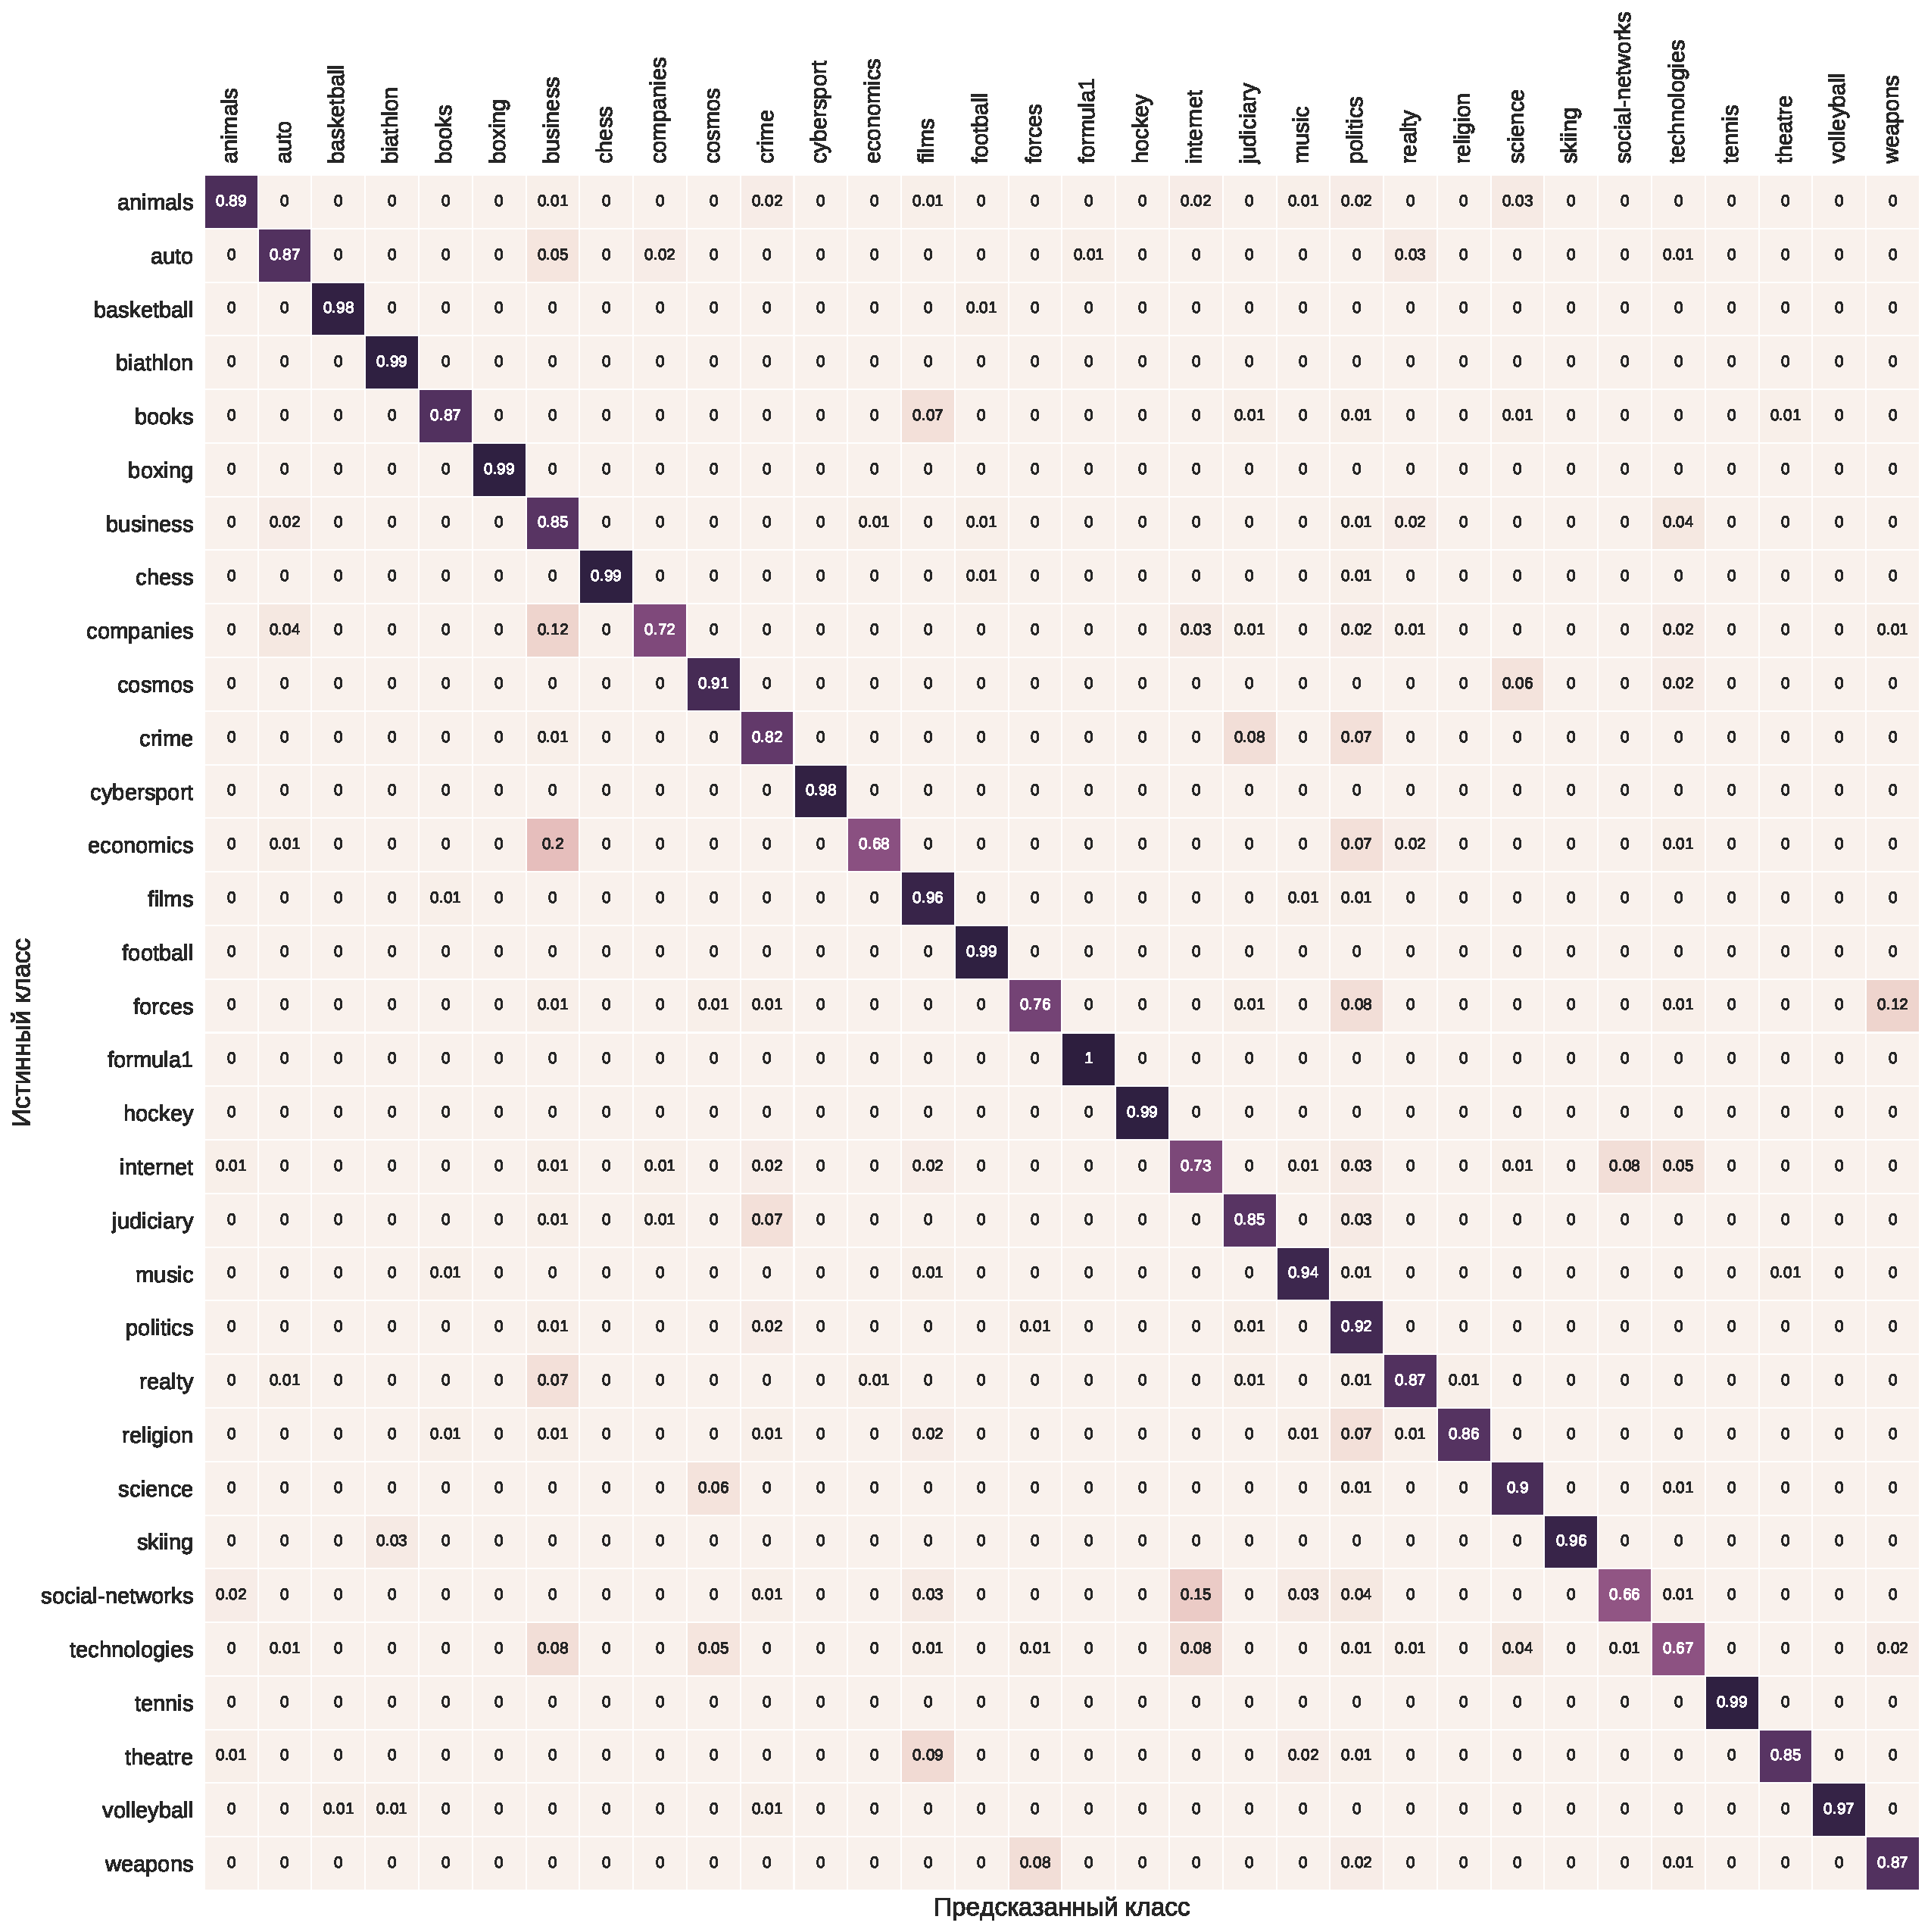
\includegraphics[width=0.95\textwidth]{svm_matrix}
	\caption{Ошибки классификатора SVM.}
	\label{svm_matrix}
\end{figure}


\begin{figure}[h!]
	\centering
	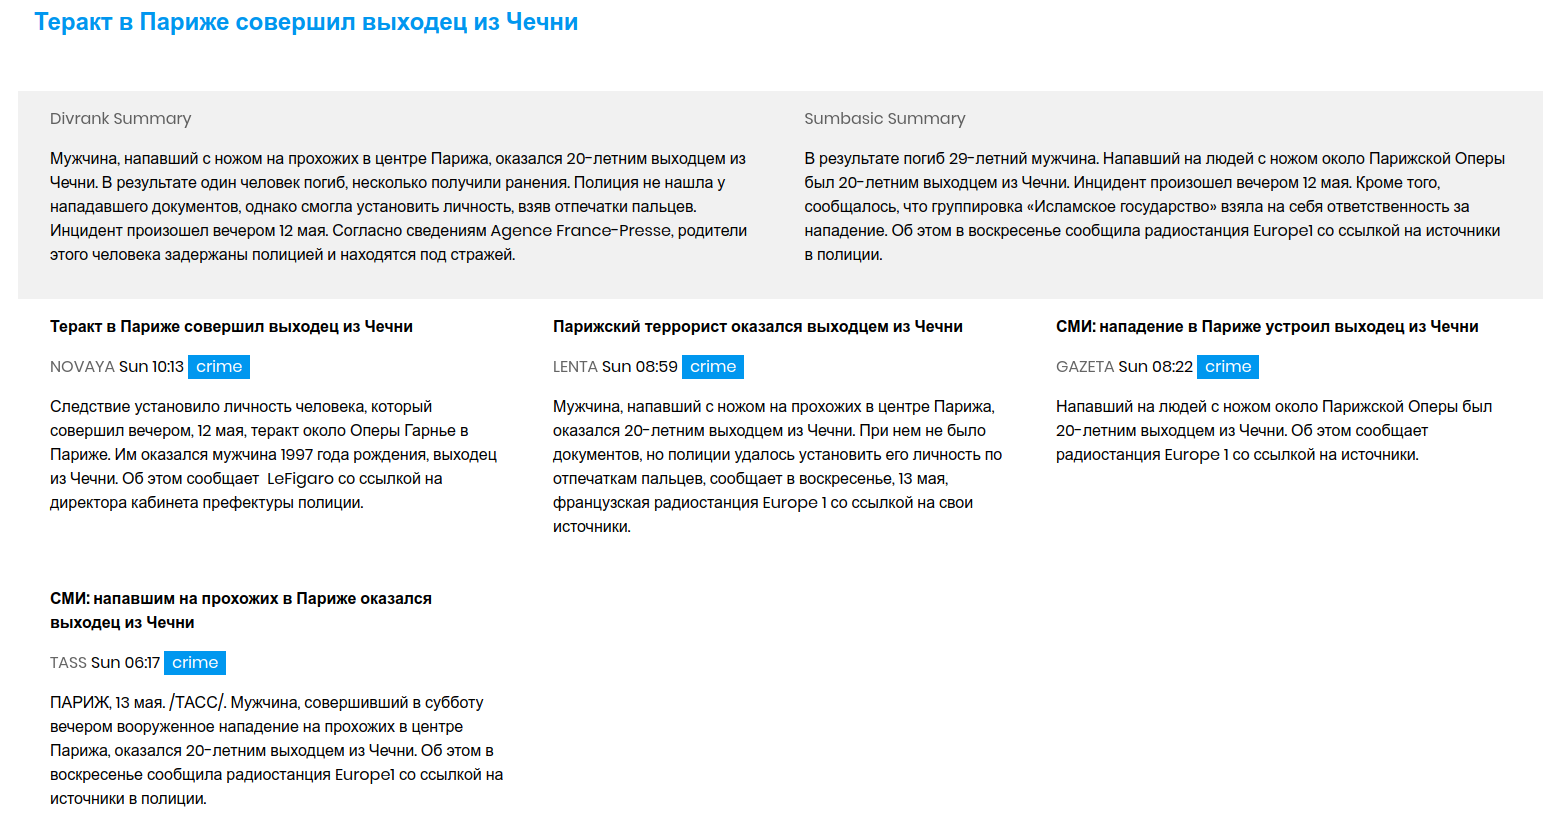
\includegraphics[width=0.95\textwidth]{var1}
	\caption{Пример функционирования сервиса 1.}
	\label{var1}
\end{figure}


\begin{figure}[h!]
	\centering
	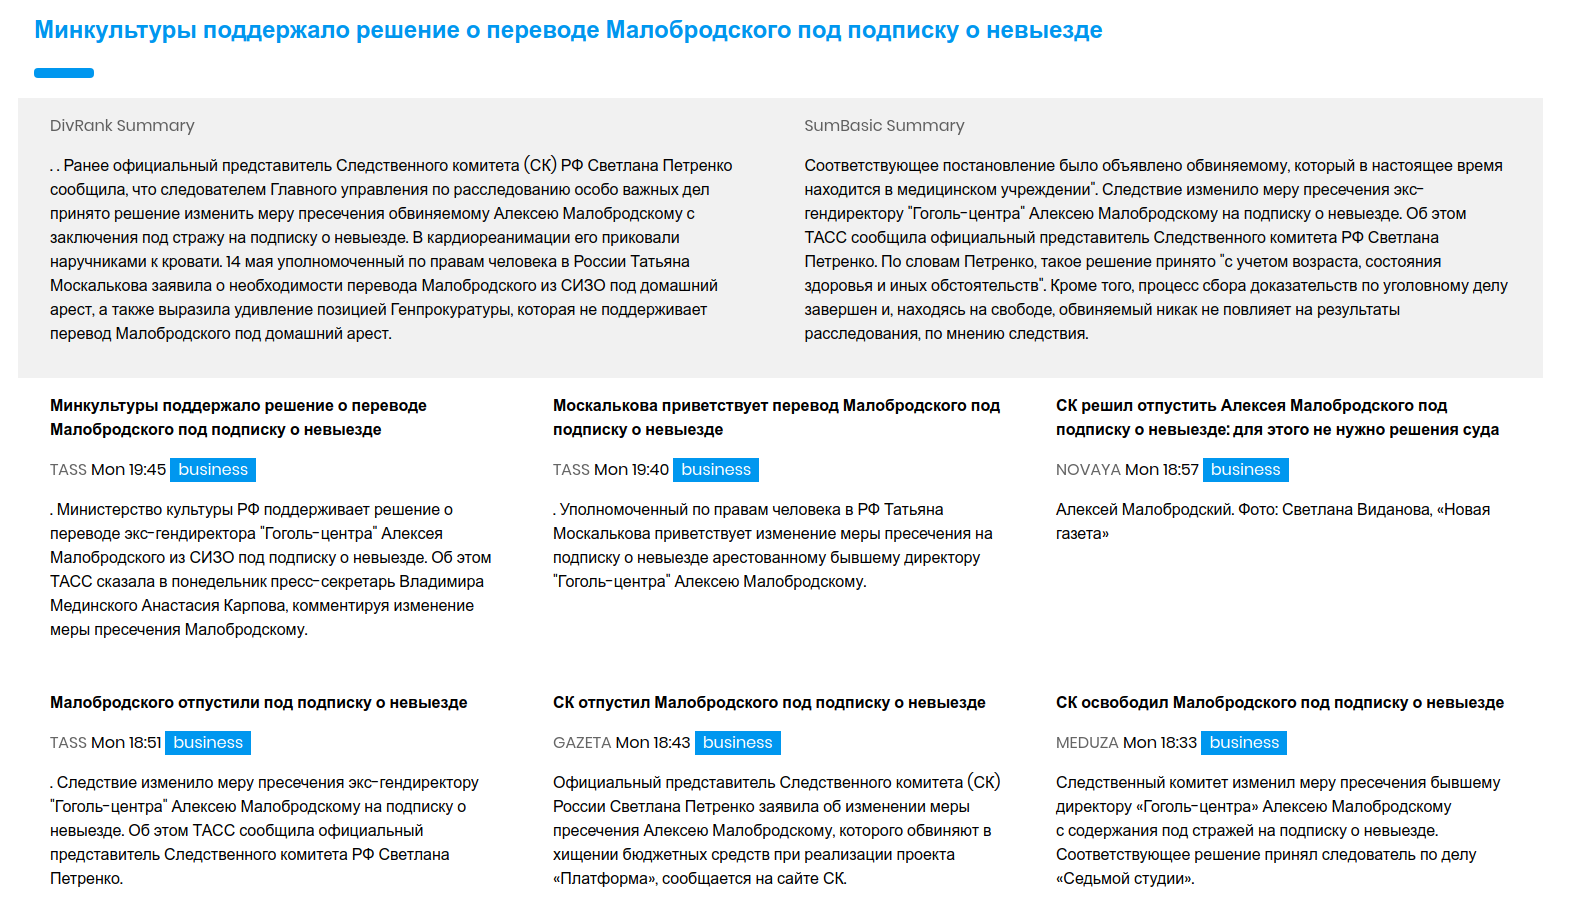
\includegraphics[width=0.95\textwidth]{var2}
	\caption{Пример функционирования сервиса 2.}
	\label{var2}
\end{figure}


\begin{figure}[h!]
	\centering
	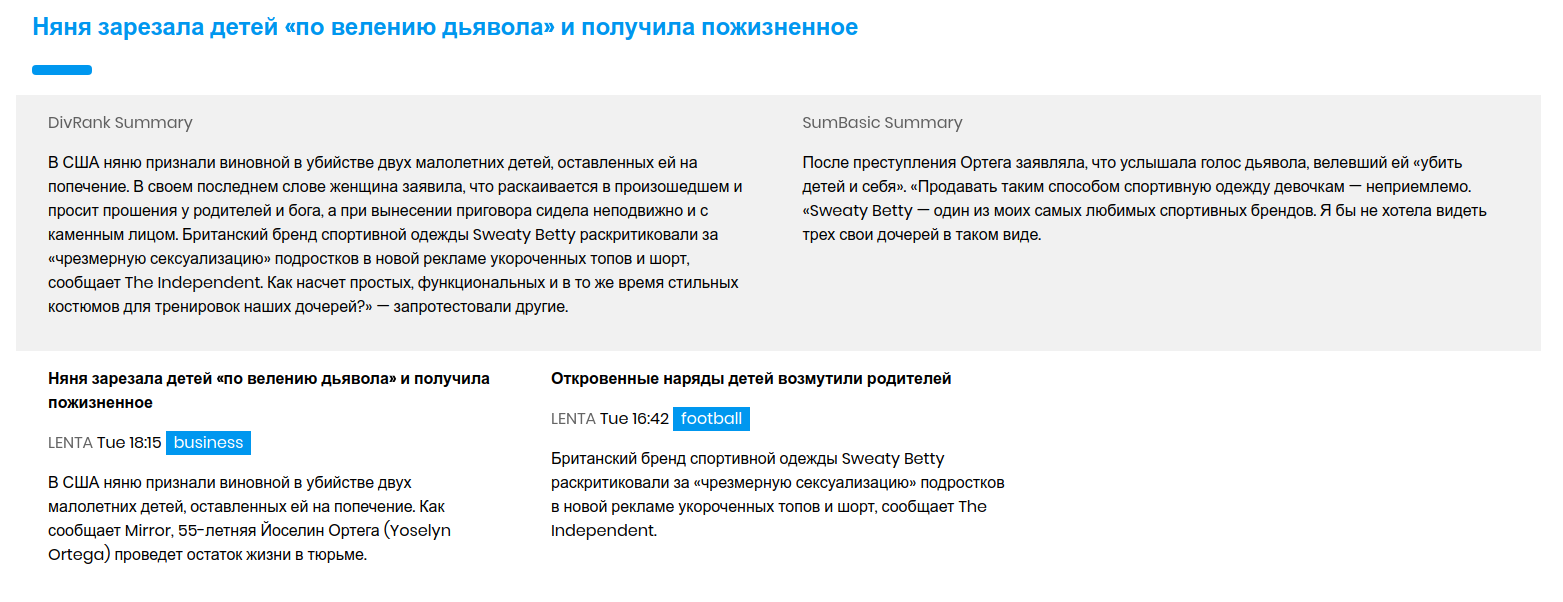
\includegraphics[width=0.95\textwidth]{var3}
	\caption{Пример функционирования сервиса 3.}
	\label{var3}
\end{figure}

\clearpage
%\begin{figure}
%	\centering
%	\begin{mdframed}[linecolor=black, topline=true, bottomline=true,
%		leftline=false, rightline=false]
	\begin{minted}[fontsize=\scriptsize]{python}
import pandas as pd
from sklearn.metrics.pairwise import cosine_similarity
import pickle
import datetime
from .normalization import TEXT_PIPELINE
from . import sum_basic, divrank
from sklearn.cluster import KMeans, MiniBatchKMeans
import time
import numpy as np
import pytz
import os

TZ = pytz.timezone('Europe/Moscow')


class Analyzer():

    """ Class-wrapper for nlp data-processing """

    def __init__(self, config={
            'kmeans': {
                'proximity_coeff': 0.6, 'n_clusters_coeff': 4,
                'batch_size': 50, 'n_init': 10, 'max_iter': 200
            },
            'append_titles': True,
            'svm_path': 'nlp/models/SVM_classifier.bin',
            'svm_labels_path': 'nlp/models/LabelEncoder.bin',
            'tfidf_path': 'nlp/models/TFIDF_vectorizer.bin',
            'max_news_distance_secs': 12*60*60,
            'drop_duplicates': True,
            'sumbasic': {
                'summary_length': 4
            },
            'divrank': {
                'summary_length': 4
            }
        }):
        self.config = config
        self._data = pd.DataFrame([])
        self._last_time = 0
        self._first_time = 0
        self._clusters = []
        self._output = []
        self._count = 0
        self.SVM = None
        self.labels = None
        self.TFIDF = None
        self._load_models()

    def fit(self, news_list):
        if not news_list:
            return
        # Cleaning and classifying new data
        new_data = self._norimalize(news_list)
        self._vectorize(new_data)
        self._classify(new_data)
        # Adding new data to existing data
        self._data = pd.concat([new_data, self._data])
        # Sorting just to be sure
        self._data.sort_values('date', inplace=True, ascending=False)
        if self.config['drop_duplicates']:
            self._data.drop_duplicates(subset='url', inplace=True)
        # Saving most recent news date for next update
        self._last_time = self._data.iloc[0].date
        self._first_time = self._data.iloc[-1].date
        # Dropping all data older then 24 hours
        self._data = self._data[self._data.date >= self._last_time - self.config['max_news_distance_secs']]
        self._count = self._data.shape[0]
        # Clusterize all data every time new data is coming
        clusters_no_sum = self._clusterize()
        self._clusters = self._summirize(clusters_no_sum)
        self._form_output()

    def get_events(self):
        return self._output

    def get_last_time(self):
        return self._form_date(self._last_time)

    def get_count(self):
        return self._count

    def _norimalize(self, news_list):
        # Converting data to pandas table
        data = pd.DataFrame(news_list)
        data = data[['media', 'url', 'title', 'text', 'topic', 'date']]
        data.date = data.date.apply(int)
        data.sort_values('date', inplace=True, ascending=False)
        # Append text_norm, title_norm columns to data w/ normalized text
        data.title = data.title.apply(lambda x: x.strip())
        data['text_norm'] = data.text.apply(TEXT_PIPELINE)
        data['title_norm'] = data.title.apply(TEXT_PIPELINE)
        return data

    def _vectorize(self, data):
        if self.config['append_titles']:
            trainX = data['title_norm']
        else:
            trainX = data['title_norm'] + ' ' + data['text_norm']
        trainX = trainX.values
        data['tfidf_vector'] = list(self.TFIDF.transform(trainX).toarray())

    def _classify(self, data):
        data['svm_class'] = list(self.SVM.predict(data['tfidf_vector'].tolist()))
        data['svm_class'] = data.apply(
            lambda row:
                self._class_to_str(row['svm_class']),
            axis=1)

    def _clusterize(self):
        config = self.config['kmeans']
        tfidf_matrix = self._data['tfidf_vector'].tolist()
        kmeans = MiniBatchKMeans(
            n_clusters=int(self._count // config['n_clusters_coeff']),
            batch_size=int(config['batch_size']),
            n_init=int(config['n_init']),
            max_iter=int(config['max_iter'])
        ).fit(tfidf_matrix)
        clusters_raw = kmeans.predict(tfidf_matrix)
        clusters = [[] for _ in range(len(clusters_raw))]
        for i, cluster in enumerate(clusters_raw):
            tfidf_news = np.array(tfidf_matrix[i]).reshape(1, -1)
            if cosine_similarity(tfidf_news,
                kmeans.cluster_centers_[cluster].reshape(1, -1))[0][0] >= self.config['kmeans']['proximity_coeff']:
                clusters[cluster].append(i)
        return self._sort_clusters(clusters)

    def _summirize(self, clusters):
        clusters_summed = []
        for news_ids in clusters:
            text = '\n'.join([self._data.iloc[id]['text'] for id in news_ids])
            try:
                divr = divrank(text, self.config['divrank'])
            except Exception as e:
                divr = ''
                print('divrank error')
            clusters_summed.append({
                'sumbasic': sum_basic(text, self.config['sumbasic']), 'divrank': divr,
                'content': news_ids
            })
        return clusters_summed

    def _load_models(self):
        with open(self.config['svm_path'], 'rb') as pickle_file:
            self.SVM = pickle.load(pickle_file)
        with open(self.config['svm_labels_path'], 'rb') as pickle_file:
            self.labels = pickle.load(pickle_file)
        with open(self.config['tfidf_path'], 'rb') as pickle_file:
            self.TFIDF = pickle.load(pickle_file)

    def _form_output(self):
        """ Creating a json output for server """
        self._output = []
        for i, cluster in enumerate(self._clusters):
            form_cluster = cluster.copy()
            form_cluster['content'] = []
            self._output.append(form_cluster)
            for id in cluster['content']:
                self._output[i]['content'].append({
                    'media': self._data.iloc[id].media,
                    'title': self._data.iloc[id].title,
                    'url': self._data.iloc[id].url,
                    'text': self._cut_text(self._data.iloc[id].text),
                    'labels': {
                        'SVM': self._data.iloc[id]['svm_class']
                    },
                    'date': self._date_to_str(self._data.iloc[id].date),
                })

    def _form_date(self, ts):
        return datetime.datetime.utcfromtimestamp(ts).replace(
            tzinfo=pytz.utc).astimezone(TZ)

    def _get_avg_time(self, group):
        avg = 0
        for n in group:
            avg += self._data.iloc[n]['date']
        return avg // len(group)

    def _sort_clusters(self, clusters):
        cs_filtered = filter(lambda x: len(x) > 1, clusters)
        # Sort by date of event
        cs_sorted = sorted(cs_filtered, key=lambda x: self._get_avg_time(x), reverse=True)
        # Sort news im cluster by time
        cs_sorted = list(map(lambda x: sorted(x,
                                           key=lambda y: self._data.iloc[y].date, reverse=True), cs_sorted))
        return cs_sorted

    def _class_to_str(self, class_num):
        """ Converting number of predicted class to string """
        return self.labels.inverse_transform(class_num)

    def _cut_text(self, text):
        """ Returns first paragraph of text """
        ps = []
        for p in text.split('\n'):
            if p != '':
                if len(p) > 500:
                    ps.append(p[:500].strip() + '...')
                    return "\n".join(ps)
                else:
                    ps.append(p.strip())
                if len(ps) == 1:
                    return "\n".join(ps)
        return ''

    def _date_to_str(self, date):
        return datetime.datetime.utcfromtimestamp(date).replace(
            tzinfo=pytz.utc).astimezone(pytz.timezone('Europe/Moscow')).strftime('%a %H:%M')

	\end{minted}
	\vspace{-1cm}
\begin{figure}[H]
	\caption{Класс \texttt{Analyzer}.}
	\label{analyzer}
\end{figure}


\begin{minted}[fontsize=\scriptsize]{python}
import requests
import re
import json
import datetime
from bs4 import BeautifulSoup
import logging
import time
import random
import os
import traceback
import pytz
from pymongo import MongoClient


logger = logging.getLogger(__name__)
if not len(logger.handlers):
    logger.setLevel(logging.INFO)
    console = logging.StreamHandler()
    formatter = logging.Formatter(
        '%(asctime)s - %(message)s', '%Y-%m-%d %H:%M:%S')
    console.setFormatter(formatter)
    console.setLevel(logging.INFO)
    logger.addHandler(console)


COLLECTION = None
def process_init():
    global COLLECTION
    db_client = MongoClient(
        'mongo',
        27017)
    db = db_client.news
    COLLECTION = db.raw_news


class BaseParser():

    """docstring for BaseParser"""

    def __init__(self, id, root_url, api_url, page_type='html'):
        self.id = id
        self.root_url = root_url  # url for news
        self.api_url = api_url  # url for pages
        self.page_type = page_type
        self.curr_date = None
        self.TZ = pytz.timezone('Europe/Moscow')

    def parse(self, pool,
                    start_time=datetime.datetime.now(), until_time=None,
                    news_count=None, topic_filter=None):
        """ Url extraction from pages in parant process """
        t_start = time.time()
        self._check_args(start_time, until_time, news_count,
                         topic_filter)
        # Some parsers do not have start time, so need to check
        start_time = start_time.timestamp()
        if until_time:
            until_time = until_time.timestamp()
        self.curr_date = start_time
        url_counter = 0
        url_to_fetch = self._page_url()
        while True:
            try:
                content = self._get_content(url_to_fetch, type_=self.page_type)
                news_list = self._get_news_list(content)
                if not news_list:
                    raise Exception('No content')
            except Exception as e:
                logger.error(
                    'Error: couldn\'t find content {} {}'.format(url_to_fetch, e))
                break

            logger.info('Look at page {}'.format(url_to_fetch))
            for news in news_list:
                try:
                    # Url always first, date always second in params
                    news_params = self._get_news_params_in_page(news)
                    if not news_params:
                        continue
                    url = news_params[0]
                    self.curr_date = news_params[1]
                    if (self.curr_date <= until_time):
                        break
                    logger.debug('push to queue ' + str(news_params))
                    pool.map_async(self._process_news, [(news_params)])
                    url_counter += 1
                    if url_counter % 10000 == 0:
                        logger .warning(
                            '{} {} news put to queue'.format(self.id, url_counter))
                except Exception as e:
                    logger.error(
                        'Error on url {}: {} '.format(url_to_fetch, traceback.format_exc()))
            else:
                url_to_fetch = self._next_page_url()
                continue
            break

        logger.info('End of parsing, time: {}'.format(
            time.strftime('%H:%M:%S', time.gmtime(time.time() - t_start))))

    def _process_news(self, news_params):
        try:
            logger.debug('pulled ' + str(news_params))
            news_out = self._parse_news(news_params)
            logger.debug('processed ' + str(news_out))
            if not news_out:
                return
            news_out['media'] = self.id
            COLLECTION.insert_one(news_out)
            logger.info('Pushed to db ' + news_out['url'])
        except Exception as err:
            logger.error("Error {} on {}".format(
                traceback.format_exc(), news_params[0]))

    def _request(self, url):
        response = requests.get(url)
        response.raise_for_status()
        return response

    def _get_content(self, url, type_='html'):
        response = self._request(url)
        if type_ == 'html':
            return BeautifulSoup(response.text.encode('utf-8'), 'lxml')
        elif type_ == 'json':
            return response.json()
        else:
            raise Exception()

    def _check_args(self, start_time, until_time,
                    news_count, topic_filter):
        pass
\end{minted}
\vspace{-1cm}
\begin{figure}[H]
	\caption{Класс \texttt{BaseParser}.}
	\label{base}
\end{figure}


\begin{minted}[fontsize=\scriptsize]{python}
import requests
import datetime
import re
from bs4 import BeautifulSoup
from .BaseParser import BaseParser
import time
import pytz


class Lenta(BaseParser):

    def __init__(self, **kwargs):
        super(Lenta, self).__init__(
            id='LENTA', root_url='https://lenta.ru',
            api_url='https://lenta.ru/news',
            page_type='html', **kwargs)

    def _get_news_list(self, content):
        """ Getting list of news from page content """
        return reversed(list(content.find_all(
            'div', 'item news b-tabloid__topic_news')))

    def _get_news_params_in_page(self, news):
        news_url = self.root_url + news.find('a')['href']
        news_date = self._str_to_time(
            self._time_to_str(self.curr_date) + ' '
            + news.find('span', 'time').text)
        return news_url, news_date

    def _page_url(self):
        # Example: https://lenta.ru/news/2017/02/01/
        return self.api_url + self._time_to_str(self.curr_date)

    def _next_page_url(self):
        self.curr_date -= int(datetime.timedelta(days=1).total_seconds())
        return self._page_url()

    def _parse_news(self, news_params):
        """ Getting full news params by direct url """
        html = self._get_content(news_params[0])
        date = news_params[1]
        title = html.find('h1', 'b-topic__title').get_text()
        paragraphs = html.find('div', attrs={"itemprop": "articleBody"})
        paragraphs = paragraphs.find_all('p')
        text = '\n'.join([p.get_text() for p in paragraphs])
        try:
            topic = html.find('a', 'b-header-inner__block')
            topic = re.match(
                r'\/rubrics\/([A-z0-9]+)\/', topic['href']).group(1)
        except Exception:
            topic = None
        try:
            tag = html.find('a', 'item dark active')
            tag = re.match(
                r'\/rubrics\/[A-z0-9]+\/(([A-z0-9]+)\/)?', tag['href']).group(2)
        except Exception:
            tag = None

        news_out = {'title': title, 'url': news_params[0], 'text': text,
                    'topic': topic, 'date': date, 'other': {'tag': tag}}
        return news_out

    def _time_to_str(self, time_):
        return datetime.datetime.utcfromtimestamp(time_).replace(
            tzinfo=pytz.utc).astimezone(self.TZ).strftime('/%Y/%m/%d/')

    def _str_to_time(self, time_str):
        return datetime.datetime.strptime(time_str, '/%Y/%m/%d/ %H:%M').replace(tzinfo=self.TZ).timestamp()

\end{minted}
\vspace{-1cm}
\begin{figure}[H]
	\caption{Пример реализации парсера \texttt{Lenta}.}
	\label{lenta}
\end{figure}


\begin{minted}[fontsize=\scriptsize]{python}
from nltk.corpus import stopwords
from stop_words import get_stop_words
from functools import lru_cache
from pymystem3 import Mystem
en_sw = get_stop_words('en')
ru_sw = get_stop_words('ru')
STOP_WORDS = set(en_sw) | set(ru_sw)
STOP_WORDS = STOP_WORDS | set(
    stopwords.words('russian')) | set(stopwords.words('english'))
STOP_WORDS = STOP_WORDS | set(['лента', 'новость', 'риа', 'тасс',
                               'редакция', 'газета', 'корра', 'daily',
                               'village', 'интерфакс', 'reuters'])

stemmer = Mystem()


class Pipeline(object):

    def __init__(self, *args):
        self.transformations = args

    def __call__(self, x):
        res = x
        for f in self.transformations:
            res = f(res)
        return res


def get_lower(text):
    return str(text).lower().strip()


def remove_punctuation(text):
    return ''.join([c if c.isalpha() or c in ['-', "'"] else ' ' for c in text])


@lru_cache(maxsize=None)
def get_word_normal_form(word):
    return ''.join(stemmer.lemmatize(word)).strip().replace('ё', 'е').strip('-')


def lemmatize_words(text):
    res = []
    for word in text.split():
        norm_form = get_word_normal_form(word)
        if len(norm_form) > 2 and norm_form not in STOP_WORDS:
            res.append(norm_form)
    return ' '.join(res)


TEXT_PIPELINE = Pipeline(get_lower, remove_punctuation, lemmatize_words)
\end{minted}
\begin{figure}[H]
	\caption{Функции нормализации \texttt{normalization}.}
	\label{normal}
\end{figure}


\begin{minted}[fontsize=\scriptsize]{python}
from flask import Flask, render_template, request,\
    redirect, url_for, jsonify
import datetime
import time
from threading import Thread
import os
from pymongo import MongoClient
import logging

logger = logging.getLogger(__name__)
if not len(logger.handlers):
    logger.setLevel(logging.INFO)
    console = logging.StreamHandler()
    formatter = logging.Formatter(
        '%(asctime)s - %(message)s', '%Y-%m-%d %H:%M:%S')
    console.setFormatter(formatter)
    console.setLevel(logging.INFO)
    logger.addHandler(console)

app = Flask(__name__, template_folder='./frontend/templates',
                      static_folder='./frontend/static',
                      static_url_path='/static')
app.config.from_object(__name__)

app.config.update(dict(
    BOOTSTRAP_WAIT=int(os.environ.get('SERVER_BOOTSTRAP_WAIT', 4*60)),
    UPDATE_RATE=int(os.environ.get('SERVER_UPDATE_RATE', 5*60)),
    OFFSET=int(os.environ.get('OFFSET', 5)),
    PORT=int(os.environ.get('PORT', 5000)),
))

db_client = MongoClient(
    'mongo',
    27017)
db = db_client.news

@app.route('/')
def index():
    return redirect(
        url_for('get_content', topic_count=5))


@app.route('/<int:topic_count>')
def get_content(topic_count=5):
    events = list(db.events.find({}))
    if len(events) < topic_count:
        return redirect(
            url_for('get_content', topic_count=len(events)))
    events_sliced = events[:topic_count]
    count = sum(len(x['content']) for x in events)
    return render_template('main.html', groups_count=len(events),
                           count=count, groups=events_sliced)


@app.route('/api/<int:offset>')
def api_get_content(offset=app.config['OFFSET']):
    events = list(db.events.find({}))
    if offset >= len(events):
        response = jsonify(message="Topic number too large")
        response.status_code = 404
        return response
    if len(events) < offset + app.config['OFFSET']:
        events = events[offset:len(events)]
    events = events[offset:offset + app.config['OFFSET']]
    return jsonify({'data': render_template('view.html', groups=events)})


@app.template_filter('min')
def reverse_filter(s):
    return min(s)


if __name__ == "__main__":
    app.run(host='0.0.0.0', port=app.config['PORT'], threaded=True, use_reloader=False)

\end{minted}
\vspace{-1cm}
\begin{figure}[H]
	\caption{Реализация сервера}
	\label{serv}
\end{figure}

\end{document}